\newpage
\thispagestyle{empty}
\mbox{}
\newpage
\thispagestyle{empty}
\thispagestyle{empty}

\setcounter{chapter}{11}
\pdfbookmark[0]{Chapter 11 Boundary Value Problems and Fourier Expansions}{chapter:11}
\chaptertitle{Boundary Value Problems and Fourier Expansions}

\noindent
IN THIS CHAPTER we develop series representations of functions
that will be used to solve partial differential equations in
Chapter~12.

\medskip\noindent
SECTION~11.1 deals with five boundary value problems
for the differential equation
$$
y''+\lambda y=0.
$$
They are related to problems in partial
differential equations that will be discussed in Chapter~12.
We define what is meant by eigenvalues and eigenfunctions of
the boundary value  problems, and  show that  the eigenfunctions have
a property called {\color{blue}\it orthogonality\/}.

\medskip\noindent
SECTION~11.2  introduces
\href{http://www-history.mcs.st-and.ac.uk/Mathematicians/Fourier.html}
{\color{blue}Fourier series},
which are  expansions
of given functions in term of sines and cosines.

\medskip\noindent
SECTION~11.3  deals with expansions of functions in terms
of the eigenfunctions of four of the eigenvalue problems discussed
in Section~11.1. They are all related to the Fourier series
discussed in Section~11.2.

\vspace*{3in}
\centerline{581}

\newpage

\section{Eigenvalue Problems for \texorpdfstring{$y''+\lambda y=0$}{y''+lambda y=0}}

\noindent
In Chapter~12 we'll study partial differential equations that arise in problems of heat conduction, wave propagation, and potential theory. The purpose of this chapter is to develop tools required to solve these equations. In this section we consider the following problems, where $\lambda$ is a real number and $L>0$:

Problem 1: \hskip5em $y''+\lambda y=0,\quad y(0)=0,\quad y(L)=0$
\medskip

Problem 2: \hskip5em $y''+\lambda y=0,\quad y'(0)=0,\quad y'(L)=0$
\medskip

Problem 3: \hskip5em $y''+\lambda y=0,\quad y(0)=0,\quad y'(L)=0$
\medskip

Problem 4: \hskip5em $y''+\lambda y=0,\quad y'(0)=0,\quad y(L)=0$
\medskip

Problem 5: \hskip5em $y''+\lambda y=0,\quad y(-L)=y(L), \quad y'(-L)=y'(L)$
\medskip

In each problem the conditions following the differential equation are called {\color{blue}\it boundary conditions\/}. Note that the boundary conditions in Problem~5, unlike those in Problems~1-4, don't require that $y$ or $y'$ be zero at the boundary points, but only that $y$ have the same value at $x=\pm L$ , and that $y'$ have the same value at $x=\pm L$. We say that the boundary conditions in Problem~5 are {\color{blue}\it periodic\/}.

Obviously, $y\equiv0$ (the trivial solution) is a solution of Problems~1-5 for any value of $\lambda$. For most values of $\lambda$, there are no other solutions. The interesting question is this:

{\color{blue}\it For what values of $\lambda$ does the problem have nontrivial solutions, and what are they?}

A value of $\lambda$ for which the problem has a nontrivial solution is an {\color{blue}\it eigenvalue\/} of the problem, and the nontrivial solutions are $\lambda$-{\color{blue}\it eigenfunctions\/}, or {\color{blue}\it eigenfunctions associated with $\lambda$\/}. Note that a nonzero constant multiple of a $\lambda$-eigenfunction is again a $\lambda$-eigenfunction.

Problems~1-5 are called {\color{blue}\it eigenvalue problems\/}. {\color{blue}\it Solving\/} an eigenvalue problem means finding all its eigenvalues and associated eigenfunctions. We'll take it as given here that all the eigenvalues of Problems~1-5 are real numbers. This is proved in a more general setting in Section~13.2.

\begin{theorem}
  \color{blue}
  \label{thmtype:11.1.1} Problems $1$--$5$ have no negative eigenvalues. Moreover, $\lambda=0$ is an eigenvalue of Problems $2$ and $5$, with associated eigenfunction $y_{0}=1$, but $\lambda=0$ isn't an eigenvalue of Problems~$1$, $3$, or $4$.
\end{theorem}

\proof We consider Problems 1-4, and leave Problem 5 to you (Exercise~\ref{exer:11.1.1}). If $y''+\lambda y=0$, then $y(y''+\lambda y)=0$, so
\[
  \int_{0}^{L}y(x)(y''(x)+\lambda y(x))\,dx=0;
\]
therefore,
\begin{equation}
  \label{eq:11.1.1}\lambda\int_{0}^{L}y^{2}(x)\,dx=-\int_{0}^{L}y(x)y''(x)\,dx.
\end{equation}
Integration by parts yields
\begin{equation}
  \label{eq:11.1.2}
  \begin{array}{rcl}
    \dst\int_{0}^{L}y(x)y''(x)\,dx & = & \dst y(x)y'(x)\lims0L-\int_{0}^{L} (y'(x))^{2}\,dx    \\
                                   & = & \dst y(L)y'(L)-y(0)y'(0)-\int_{0}^{L}(y'(x))^{2}\,dx.
  \end{array}
\end{equation}
However, if $y$ satisfies any of the boundary conditions of Problems 1-4, then
\[
  y(L)y'(L)-y(0)y'(0)=0;
\]
hence, \eqref{eq:11.1.1} and \eqref{eq:11.1.2} imply that
\[
  \lambda\int_{0}^{L}y^{2}(x)\,dx=\int_{0}^{L}(y'(x))^{2}\,dx.
\]
If $y\not\equiv0$, then $\int_{0}^{L}y^{2}(x)\,dx>0$. Therefore $\lambda\ge0$ and, if $\lambda=0$, then $y'(x)=0$ for all $x$ in $(0,L)$ (why?), and $y$ is constant on $(0,L)$. Any constant function satisfies the boundary conditions of Problem~2, so $\lambda=0$ is an eigenvalue of Problem~2 and any nonzero constant function is an associated eigenfunction. However, the only constant function that satisfies the boundary conditions of Problems $1$, $3$, or $4$ is $y\equiv0$. Therefore $\lambda=0$ isn't an eigenvalue of any of these problems.

\begin{example}[Problem 1]
  \label{example:11.1.1} \rm Solve the eigenvalue problem
  \begin{equation}
    \label{eq:11.1.3}y''+\lambda y=0,\quad y(0)=0,\quad y(L)=0.
  \end{equation}

  \solution From Theorem~\ref{thmtype:11.1.1}, any eigenvalues of \eqref{eq:11.1.3} must be positive. If $y$ satisfies \eqref{eq:11.1.3} with $\lambda>0$, then
  \[
    y=c_{1}\cos\sqrt{\lambda}\,x+c_{2}\sin\sqrt{\lambda}\,x,
  \]
  where $c_{1}$ and $c_{2}$ are constants. The boundary condition $y(0)=0$ implies that $c_{1}=0$. Therefore $y=c_{2}\sin\sqrt{\lambda}\,x$. Now the boundary condition $y(L)=0$ implies that $c_{2}\sin\sqrt{\lambda}\,L=0$. To make $c_{2}\sin\sqrt{\lambda}\,L=0$ with $c_{2}\ne0$, we must choose $\sqrt{\lambda}=n\pi/L$, where $n$ is a positive integer. Therefore $\lambda_{n}=n^{2}\pi^{2}/L^{2}$ is an eigenvalue and
  \[
    y_{n}=\sin\frac{n\pi x}{L}
  \]
  is an associated eigenfunction. \bbox
\end{example}

For future reference, we state the result of Example~\ref{example:11.1.1} as a theorem.

\begin{theorem}
  \color{blue}
  \label{thmtype:11.1.2} The eigenvalue problem
  \[
    y''+\lambda y=0,\quad y(0)=0,\quad y(L)=0
  \]
  has infinitely many positive eigenvalues $\lambda_{n}=n^{2}\pi^{2}/L^{2}$, with associated eigenfunctions
  \[
    y_{n}=\sin\frac{n\pi x}{L},\quad n=1,2,3,\dots.
  \]
  There are no other eigenvalues.
\end{theorem}

We leave it to you to prove the next theorem about Problem~2 by an argument like that of Example~\ref{example:11.1.1} (Exercise~\ref{exer:11.1.17}).

\begin{theorem}
  \color{blue}
  \label{thmtype:11.1.3} The eigenvalue problem
  \[
    y''+\lambda y=0,\quad y'(0)=0,\quad y'(L)=0
  \]
  has the eigenvalue $\lambda_{0}=0$, with associated eigenfunction $y_{0}=1$, and infinitely many positive eigenvalues $\lambda_{n}=n^{2}\pi^{2}/L^{2}$, with associated eigenfunctions
  \[
    y_{n}=\cos\frac{n\pi x}{L},n=1,2,3\dots.
  \]
  There are no other eigenvalues.
\end{theorem}

\begin{example}[Problem 3]
  \label{example:11.1.2} \rm Solve the eigenvalue problem
  \begin{equation}
    \label{eq:11.1.4}y''+\lambda y=0,\quad y(0)=0,\quad y'(L)=0.
  \end{equation}

  \solution From Theorem~\ref{thmtype:11.1.1}, any eigenvalues of \eqref{eq:11.1.4} must be positive. If $y$ satisfies \eqref{eq:11.1.4} with $\lambda>0$, then
  \[
    y=c_{1}\cos\sqrt{\lambda}\,x+c_{2}\sin\sqrt{\lambda}\,x,
  \]
  where $c_{1}$ and $c_{2}$ are constants. The boundary condition $y(0)=0$ implies that $c_{1}=0$. Therefore $y=c_{2}\sin\sqrt{\lambda}\,x$. Hence, $y'=c_{2}\sqrt{\lambda}\cos\sqrt{\lambda}\,x$ and the boundary condition $y'(L)=0$ implies that $c_{2}\cos\sqrt{\lambda}\,L=0$. To make $c_{2}\cos\sqrt{\lambda}\,L=0$ with $c_{2}\ne0$ we must choose
  \[
    \sqrt{\lambda}=\frac{(2n-1)\pi}{2L},
  \]
  where $n$ is a positive integer. Then $\lambda_{n}=(2n-1)^{2}\pi^{2}/4L^{2}$ is an eigenvalue and
  \[
    y_{n}=\sin\frac{(2n-1)\pi x}{2L}
  \]
  is an associated eigenfunction. \bbox
\end{example}

For future reference, we state the result of Example~\ref{example:11.1.2} as a theorem.

\begin{theorem}
  \color{blue}
  \label{thmtype:11.1.4} The eigenvalue problem
  \[
    y''+\lambda y=0,\quad y(0)=0,\quad y'(L)=0
  \]
  has infinitely many positive eigenvalues $\lambda_{n}=(2n-1)^{2}\pi^{2}/4L^{2}$, with associated eigenfunctions
  \[
    y_{n}=\sin\frac{(2n-1)\pi x}{2L},\quad n=1,2,3,\dots.
  \]
  There are no other eigenvalues.
\end{theorem}

We leave it to you to prove the next theorem about Problem~4 by an argument like that of Example~\ref{example:11.1.2} (Exercise~\ref{exer:11.1.18}).

\begin{theorem}
  \color{blue}
  \label{thmtype:11.1.5} The eigenvalue problem
  \[
    y''+\lambda y=0,\quad y'(0)=0,\quad y(L)=0
  \]
  has infinitely many positive eigenvalues $\lambda_{n}=(2n-1)^{2}\pi^{2}/4L^{2}$, with associated eigenfunctions
  \[
    y_{n}=\cos\frac{(2n-1)\pi x}{2L},\quad n=1,2,3,\dots.
  \]
  There are no other eigenvalues.
\end{theorem}

\begin{example}[Problem 5]
  \label{example:11.1.3} \rm Solve the eigenvalue problem
  \begin{equation}
    \label{eq:11.1.5}y''+\lambda y=0,\quad y(-L)=y(L),\quad y'(-L)=y'(L).
  \end{equation}

  \solution From Theorem~\ref{thmtype:11.1.1}, $\lambda=0$ is an eigenvalue of \eqref{eq:11.1.5} with associated eigenfunction $y_{0}=1$, and any other eigenvalues must be positive. If $y$ satisfies \eqref{eq:11.1.5} with $\lambda>0$, then
  \begin{equation}
    \label{eq:11.1.6}y=c_{1}\cos\sqrt{\lambda}\,x+c_{2}\sin\sqrt{\lambda}\,x,
  \end{equation}
  where $c_{1}$ and $c_{2}$ are constants. The boundary condition $y(-L)=y(L)$ implies that
  \begin{equation}
    \label{eq:11.1.7}c_{1}\cos(-\sqrt{\lambda}\,L)+c_{2}\sin(-\sqrt{\lambda}\,L)=c_{1}\cos\sqrt{\lambda}\,L+c_{2}\sin\sqrt{\lambda}\,L.
  \end{equation}
  Since
  \begin{equation}
    \label{eq:11.1.8}\cos(-\sqrt{\lambda}\,L)=\cos\sqrt{\lambda}\,L\mbox{\quad and \quad}\sin(-\sqrt{\lambda}\,L)=-\sin\sqrt{\lambda}\,L,
  \end{equation}
  \eqref{eq:11.1.7} implies that
  \begin{equation}
    \label{eq:11.1.9}c_{2}\sin\sqrt{\lambda}\,L=0.
  \end{equation}
  Differentiating \eqref{eq:11.1.6} yields
  \[
    y'=\sqrt{\lambda}\left(-c_{1}\sin\sqrt{\lambda}x+c_{2}\cos\sqrt{\lambda}x\right).
  \]
  The boundary condition $y'(-L)=y'(L)$ implies that
  \[
    -c_{1}\sin(-\sqrt{\lambda}\,L)+c_{2}\cos(-\sqrt{\lambda}\,L)=-c_{1}\sin\sqrt{\lambda}\,L+c_{2}\cos\sqrt{\lambda}\,L,
  \]
  and \eqref{eq:11.1.8} implies that
  \begin{equation}
    \label{eq:11.1.10}c_{1}\sin\sqrt{\lambda}\,L=0.
  \end{equation}

  Eqns.~\eqref{eq:11.1.9} and \eqref{eq:11.1.10} imply that $c_{1}=c_{2}=0$ unless $\sqrt{\lambda}=n\pi/L$, where $n$ is a positive integer. In this case \eqref{eq:11.1.9} and \eqref{eq:11.1.10} both hold for arbitrary $c_{1}$ and $c_{2}$. The eigenvalue determined in this way is $\lambda_{n}=n^{2}\pi^{2}/L^{2}$, and each such eigenvalue has the linearly independent associated eigenfunctions
  \[
    \cos\frac{n\pi x}{L}\mbox{\quad and \quad}\sin\frac{n\pi x}{L}. \eqno{\bbox}
  \]
\end{example}

For future reference we state the result of Example~\ref{example:11.1.3} as a theorem.

\begin{theorem}
  \color{blue}
  \label{thmtype:11.1.6} The eigenvalue problem
  \[
    y''+\lambda y=0,\quad y(-L)=y(L),\quad y'(-L)=y'(L),
  \]
  has the eigenvalue $\lambda_{0}=0$, with associated eigenfunction $y_{0}=1$ and infinitely many positive eigenvalues $\lambda_{n}=n^{2}\pi^{2}/L^{2}$, with associated eigenfunctions
  \[
    y_{1n}=\cos\frac{n\pi x}{L}\mbox{\quad and \quad}y_{2n}=\sin\frac{n\pi x}{L},\quad n=1,2,3,\dots.
  \]
  There are no other eigenvalues.
\end{theorem}

\boxit{Orthogonality}

\noindent
We say that two integrable functions $f$ and $g$ are {\color{blue}\it orthogonal\/} on an interval $[a,b]$ if
\[
  \int_{a}^{b}f(x)g(x)\,dx=0.
\]
More generally, we say that the functions $\phi_{1}$, $\phi_{2}$, \dots, $\phi_{n}$, \dots (finitely or infinitely many) are orthogonal on $[a,b]$ if
\[
  \int_{a}^{b}\phi_{i}(x)\phi_{j}(x)\,dx=0\mbox{\quad whenever \quad}i\ne j.
\]
The importance of orthogonality will become clear when we study Fourier series in the next two sections.

\begin{example}
  \label{example:11.1.4} \rm Show that the eigenfunctions
  \begin{equation}
    \label{eq:11.1.11}1,\,\cos\frac{\pi x}{L},\,\sin\frac{\pi x}{L}, \,\cos\frac{2\pi x}{L},\,\sin\frac{2\pi x}{L},\dots, \cos\frac{n\pi x}{L},\,\sin\frac{n\pi x}{L},\dots
  \end{equation}
  of Problem 5 are orthogonal on $[-L,L]$.
\end{example}

\solution We must show that
\begin{equation}
  \label{eq:11.1.12}\int_{-L}^{L}f(x)g(x)\,dx=0
\end{equation}
whenever $f$ and $g$ are distinct functions from \eqref{eq:11.1.11}. If $r$ is any nonzero integer, then
\begin{equation}
  \label{eq:11.1.13}\int_{-L}^{L}\cos\frac{r\pi x}{L}\,dx =\frac{L}{r\pi}\sin\frac{r\pi x}{L}\bigg|_{-L}^{L}=0.
\end{equation}
and
\[
  \int_{-L}^{L}\sin\frac{r\pi x}{L}\,dx =-\frac{L}{r\pi}\cos\frac{r\pi x}{L}\bigg|_{-L}^{L}=0.
\]
Therefore \eqref{eq:11.1.12} holds if $f\equiv1$ and $g$ is any other function in \eqref{eq:11.1.11}.

If $f(x)=\cos m\pi x/L$ and $g(x)=\cos n\pi x/L$ where $m$ and $n$ are distinct positive integers, then
\begin{equation}
  \label{eq:11.1.14}\int_{-L}^{L}f(x)g(x)\,dx=\int_{-L}^{L}\cos\frac{m\pi x}{L}\cos\frac{n\pi x}{L}\,dx.
\end{equation}
To evaluate this integral, we use the identity
\[
  \cos A\cos B=\frac{1}{2}[\cos(A-B)+\cos(A+B)]
\]
with $A=m\pi x/L$ and $B=n\pi x/L$. Then \eqref{eq:11.1.14} becomes
\[
  \int_{-L}^{L}f(x)g(x)\,dx=\frac{1}{2}\left[\int_{-L}^{L}\cos\frac{(m-n)\pi x}{L}\,dx +\int_{-L}^{L}\cos\frac{(m+n)\pi x}{L}\,dx\right].
\]
Since $m-n$ and $m+n$ are both nonzero integers, \eqref{eq:11.1.13} implies that the integrals on the right are both zero. Therefore \eqref{eq:11.1.12} is true in this case.

If $f(x)=\sin m\pi x/L$ and $g(x)=\sin n\pi x/L$ where $m$ and $n$ are distinct positive integers, then
\begin{equation}
  \label{eq:11.1.15}\int_{-L}^{L}f(x)g(x)\,dx=\int_{-L}^{L}\sin\frac{m\pi x}{L}\sin\frac{n\pi x}{L}\,dx.
\end{equation}
To evaluate this integral, we use the identity
\[
  \sin A\sin B=\frac{1}{2}[\cos(A-B)-\cos(A+B)]
\]
with $A=m\pi x/L$ and $B=n\pi x/L$. Then \eqref{eq:11.1.15} becomes
\[
  \int_{-L}^{L}f(x)g(x)\,dx=\frac{1}{2}\left[\int_{-L}^{L}\cos\frac{(m-n)\pi x}{L}\,dx -\int_{-L}^{L}\cos\frac{(m+n)\pi x}{L}\,dx\right]=0.
\]

If $f(x)=\sin m\pi x/L$ and $g(x)=\cos n\pi x/L$ where $m$ and $n$ are positive integers (not necessarily distinct), then
\[
  \int_{-L}^{L}f(x)g(x)\,dx=\int_{-L}^{L}\sin\frac{m\pi x}{L}\cos\frac{n\pi x}{L}\,dx=0
\]
because the integrand is an odd function and the limits are symmetric about $x=0$. \bbox

Exercises~\ref{exer:11.1.19}-\ref{exer:11.1.22} ask you to verify that the eigenfunctions of Problems~1-4 are orthogonal on $[0,L]$. However, this also follows from a general theorem that we'll prove in Chapter~13.

%\end{comment}

\exercises

\begin{exerciselist}
  \item\label{exer:11.1.1} Prove that $\lambda=0$ is an eigenvalue of Problem~5 with associated eigenfunction $y_{0}=1$, and that any other eigenvalues must be positive. \hint{See the proof of Theorem~\ref{thmtype:11.1.1}.}

  \exercisetext{In Exercises 2-16 solve the eigenvalue problem.}

  \item\label{exer:11.1.2} $y''+\lambda y=0,\quad y(0)=0,\quad y(\pi)=0$

  \item\label{exer:11.1.3} $y''+\lambda y=0,\quad y'(0)=0,\quad y'(\pi)=0$

  \item\label{exer:11.1.4} $y''+\lambda y=0$,\quad $y(0)=0$,\quad $y'(\pi)=0$

  \item\label{exer:11.1.5} $y''+\lambda y=0$,\quad $y'(0)=0$,\quad $y(\pi)=0$

  \item\label{exer:11.1.6} $y''+\lambda y=0,\quad y(-\pi)=y(\pi),\quad y'(-\pi)=y'(\pi)$

  \item\label{exer:11.1.7} $y''+\lambda y=0,\quad y'(0)=0,\quad y'(1)=0$

  \item\label{exer:11.1.8} $y''+\lambda y=0$,\quad $y'(0)=0$,\quad $y(1)=0$

  \item\label{exer:11.1.9} $y''+\lambda y=0,\quad y(0)=0,\quad y(1)=0$

  \item\label{exer:11.1.10} $y''+\lambda y=0,\quad y(-1)=y(1),\quad y'(-1)=y'(1)$

  \item\label{exer:11.1.11} $y''+\lambda y=0$,\quad $y(0)=0$,\quad $y'(1)=0$

  \item\label{exer:11.1.12} $y''+\lambda y=0,\quad y(-2)=y(2),\quad y'(-2)=y'(2)$

  \item\label{exer:11.1.13} $y''+\lambda y=0,\quad y(0)=0,\quad y(2)=0$

  \item\label{exer:11.1.14} $y''+\lambda y=0$,\quad $y'(0)=0$,\quad $y(3)=0$

  \item\label{exer:11.1.15} $y''+\lambda y=0$,\quad $y(0)=0$,\quad $y'(1/2)=0$

  \item\label{exer:11.1.16} $y''+\lambda y=0,\quad y'(0)=0,\quad y'(5)=0$

  \item\label{exer:11.1.17} Prove Theorem~\ref{thmtype:11.1.3}.

  \item\label{exer:11.1.18} Prove Theorem~\ref{thmtype:11.1.5}.

  \item\label{exer:11.1.19} Verify that the eigenfunctions
  \[
    \sin\frac{\pi x}{L}, \,\sin\frac{2\pi x}{L},\dots, \,\sin\frac{n\pi x}{L},\dots\,
  \]
  of Problem~1 are orthogonal on $[0,L]$.

  \item\label{exer:11.1.20} Verify that the eigenfunctions
  \[
    1,\,\cos\frac{\pi x}{L}, \,\cos\frac{2\pi x}{L},\dots, \,\cos\frac{n\pi x}{L},\dots\,
  \]
  of Problem~2 are orthogonal on $[0,L]$.

  \item\label{exer:11.1.21} Verify that the eigenfunctions
  \[
    \sin\frac{\pi x}{2L}, \,\sin\frac{3\pi x}{2L},\dots, \,\sin\frac{(2n-1)\pi x}{2L},\dots\,
  \]
  of Problem~3 are orthogonal on $[0,L]$.

  \item\label{exer:11.1.22} Verify that the eigenfunctions
  \[
    \cos\frac{\pi x}{2L}, \,\cos\frac{3\pi x}{2L},\dots, \,\cos\frac{(2n-1)\pi x}{2L},\dots\,
  \]
  of Problem~4 are orthogonal on $[0,L]$.

  \exercisetext{In Exercises~\ref{exer:11.1.23}-\ref{exer:11.1.26} solve the eigenvalue problem.}

  \item\label{exer:11.1.23} $y''+\lambda y=0,\quad y(0)=0,\quad\dst\int_{0}^{L}y(x)\,dx=0$

  \item\label{exer:11.1.24} $y''+\lambda y=0,\quad y'(0)=0,\quad\dst\int_{0}^{L}y(x)\,dx=0$

  \item\label{exer:11.1.25} $y''+\lambda y=0,\quad y(L)=0,\quad\dst\int_{0}^{L}y(x)\,dx=0$

  \item\label{exer:11.1.26} $y''+\lambda y=0,\quad y'(L)=0,\quad\dst\int_{0}^{L}y(x)\,dx=0$
\end{exerciselist}


\newsection{2} {Boundary Value Problems and Fourier Expansions}
{Fourier Expansions I}
\currentpdfbookmark{Section 11.2 Fourier Expansions I}{section:11.2}
\vskip14pt

\renewcommand{\thissection}{\sectiontitle
{\,FOURIER EXPANSIONS I\quad}}
\thissection

\noindent
In Example~\ref{example:11.1.4} and
Exercises~11.1.~\hspace*{-3pt}\ref{exer:11.1.4}--11.1.~\hspace*{-3pt}\ref{exer:11.1.22} we saw
that the
  eigenfunctions of Problem~5 are orthogonal on $[-L,L]$ and the
eigenfunctions of Problems~1--4 are orthogonal on $[0,L]$.
In this section and the next we introduce some series expansions
in terms of these eigenfunctions.
We'll use these expansions  to solve partial differential equations in
Chapter~12.

\begin{theorem}\color{blue} \label{thmtype:11.2.1}
Suppose the functions  $\phi_1,$ $\phi_2,$
$\phi_3,$ \dots$,$ are orthogonal on $[a,b]$ and
\begin{equation} \label{eq:11.2.1}
\int_a^b\phi_n^2(x)\,dx\ne0,\quad n=1,2,3,\dots.
\end{equation}
Let $c_1,$ $c_2,$ $c_3,$\dots  be constants such that the partial sums
$f_N(x)=\sum_{m=1}^N c_m\phi_m(x)$ satisfy the inequalities
$$
|f_N(x)|\le M,\quad a\le x\le b,\quad N=1,2,3,\dots
$$
for some constant $M<\infty.$ Suppose  also that
the series
\begin{equation} \label{eq:11.2.2}
f(x)=\sum_{m=1}^\infty c_m\phi_m(x)
\end{equation}
converges and is integrable on $[a,b]$.
Then
\begin{equation} \label{eq:11.2.3}
c_n={\dst\int_a^bf(x)\phi_n(x)\,dx\over\dst\int_a^b\phi_n^2(x)\,dx},\quad
n=1,2,3,\dots.
\end{equation}
\end{theorem}

\proof Multiplying \eqref{eq:11.2.2} by $\phi_n$ and
integrating yields
\begin{equation} \label{eq:11.2.4}
\int_a^b f(x)\phi_n(x)\,dx=\int_a^b
\phi_n(x)\left(\sum_{m=1}^\infty c_m\phi_m(x)\right)\,dx.
\end{equation}
It can be shown that the
 boundedness of the partial sums
$\{f_N\}_{N=1}^\infty$ and the integrability of $f$
allow us to interchange the operations of integration and summation
on the right of \eqref{eq:11.2.4}, and rewrite \eqref{eq:11.2.4} as
\begin{equation} \label{eq:11.2.5}
\int_a^b f(x)\phi_n(x)\,dx=\sum_{m=1}^\infty c_m
\int_a^b\phi_n(x) \phi_m(x)\,dx.
\end{equation}
(This isn't  easy to prove.) Since
$$
\int_a^b\phi_n(x)\phi_m(x)\,dx=0\mbox{\quad if \quad}m\ne n,
$$
\eqref{eq:11.2.5} reduces to
$$
\int_a^bf(x) \phi_n(x)\,dx=c_n\int_a^b\phi_n^2(x)\,dx.
$$
Now  \eqref{eq:11.2.1} implies \eqref{eq:11.2.3}.\bbox

Theorem~\ref{thmtype:11.2.1} motivates the next
definition.

\begin{definition}\color{blue}\label{thmtype:11.2.2} \rm
Suppose
$\phi_1,$ $\phi_2$, \dots, $\phi_n$,\dots are
orthogonal on $[a,b]$ and
$\int_a^b\phi_n^2(x)\,dx\ne0$, $n=1$, $2$, $3$, \dots. Let
$f$ be integrable on $[a,b],$ and define
\begin{equation} \label{eq:11.2.6}
c_n={\dst\int_a^bf(x)\phi_n(x)\,dx\over\dst\int_a^b\phi_n^2(x)\,dx},\quad
n=1,2,3,\dots.
\end{equation}
Then the infinite series
$\sum_{n=1}^\infty c_n\phi_n(x)$ is called the {\color{blue}\it
Fourier expansion of $f$ in terms
of the orthogonal set\/} $\{\phi_n\}_{n=1}^\infty$, and
$c_1$, $c_2$, \dots, $c_n$, \dots
are called the {\color{blue}\it Fourier coefficients of $f$\/ with respect to\/}
$\{\phi_n\}_{n=1}^\infty$. We indicate the relationship between $f$
and its Fourier
 expansion by
\begin{equation} \label{eq:11.2.7}
f(x)\sim\sum_{n=1}^\infty c_n\phi_n(x),\quad  a\le x\le b.
\end{equation}
\end{definition}

You may wonder why we don't write
$$
f(x)=\sum_{n=1}^\infty c_n\phi_n(x),\quad  a\le x\le b,
$$
rather than \eqref{eq:11.2.7}.
Unfortunately, this isn't always true. The series on the right
may diverge for some or all values
of $x$ in $[a,b]$, or it may converge to $f(x)$ for some values of
$x$ and not for others.  So, for now,  we'll just think of the series
as being associated with $f$ because of the definition
of the coefficients $\{c_n\}$, and we'll indicate
this association informally as in \eqref{eq:11.2.7}.

\newpage
\boxit{Fourier Series}

\noindent
We'll now study Fourier expansions in terms
 of the eigenfunctions
$$
1,\, \cos{\pi x\over L},\, \sin{\pi x\over L},
\, \cos{2\pi x\over L}, \, \sin{2\pi x\over L},\dots,
\cos{n\pi x\over L}, \, \sin{n\pi x\over L},\dots.
$$
of Problem~5.
 If $f$ is integrable on $[-L,L]$,  its
Fourier expansion in terms of these functions is called the {\color{blue}\it
Fourier series of $f$ on $[-L,L]$\/}.  Since
$$
\int_{-L}^L 1^2\,dx=2L,
$$
$$
\int_{-L}^L\cos^2{n\pi x\over L}\,dx =
{1\over2}\int_{-L}^L\left(1+\cos{2n\pi x\over L}\right)\,dx=
{1\over2}\left(x+{L\over2n\pi}\sin{2n\pi x\over L}\right)
\lims{-L}L=L,
$$
and
$$
\int_{-L}^L\sin^2{n\pi x\over L}\,dx =
{1\over2}\int_{-L}^L\left(1-\cos{2n\pi x\over L}\right)\,dx=
{1\over2}\left(x-{L\over2n\pi}\sin{2n\pi x\over L}\right),
\lims{-L}L=L,
$$
we see from \eqref{eq:11.2.6} that the Fourier series of $f$ on $[-L,L]$ is
$$
 a_0+\sum_{n=1}^\infty \left(a_n\cos{n\pi x\over
L}+b_n\sin{n\pi x\over L}\right),
$$
where
$$
a_0={1\over 2L}\int_{-L}^L f(x)\,dx,
$$
$$
a_n= {1\over L}\int_{-L}^L f(x)\cos{n\pi
x\over L}\,dx,\mbox{\quad and \quad}
b_n={1\over L}\int_{-L}^L f(x)\sin{n\pi x\over L}\,dx,\,n\ge1.
$$

Note that
$a_0$ is the average value of $f$ on $[-L,L]$, while $a_n$ and $b_n$
(for $n\ge1$) are twice the average values of
$$
f(x)\cos{n\pi x\over L}\quad\mbox{ and }\quad f(x)\sin{n\pi x\over L}
$$
on $[-L,L]$, respectively.

\boxit{Convergence of Fourier Series}

\noindent
The  question of convergence of Fourier series for arbitrary
integrable functions is beyond the scope of this book. However, we can
state a theorem that settles this question for most functions that
arise in applications.

\begin{definition}\color{blue} \label{thmtype:11.2.3}\rm
A function  $f$ is said to be
  {\color{blue}\it piecewise smooth\/} on $[a,b]$ if:
\begin{alist}
\item % (a)
$f$ has at most finitely many points of discontinuity in $(a,b)$;
\item % (b)
$f'$ exists and is continuous except possibly at finitely many points
in $(a,b)$;
\item % (c)
$f(x_0+)=\lim_{x\to x_0+}f(x)$ and
$f'(x_0+)=\lim_{x\to x_0+}f'(x)$ exist if $a\le x_0<b$;
\item % (d)
$f(x_0-)=\lim_{x\to x_0-}f(x)$ and
$f'(x_0-)=\lim_{x\to x_0-}f'(x)$ exist if  $a< x_0\le b$.
\end{alist}
\end{definition}

Since $f$ and $f'$ are required to be continuous at all but
finitely many points in $[a,b]$,
 $f(x_0+)=f(x_0-)$
and $f'(x_0+)=f'(x_0-)$ for all but finitely many
values of $x_0$ in $(a,b)$. Recall from Section~8.1 that
$f$ is said to have a {\color{blue}\it jump discontinuity\/} at $x_0$
if $f(x_0+)\ne f(x_0-)$.

The next theorem gives sufficient conditions for convergence of a
Fourier series. The  proof is beyond the scope of this book.

\begin{theorem}\color{blue} \label{thmtype:11.2.4}
If $f$ is piecewise smooth on $[-L,L]$, then the Fourier series
\begin{equation} \label{eq:11.2.8}
F(x)=a_0+\sum_{n=1}^\infty\left(a_n\cos{n\pi x\over L}+b_n\sin{n\pi
x\over L}\right)
\end{equation}
of $f$
on $[-L,L]$ converges for all $x$ in $[-L,L];$ moreover$,$
$$
F(x)=
\left\{\begin{array}{cl}
f(x)&\mbox{if $-L<x<L$ and $f$ is continuous at $x$  }\\[2\jot]
\dst{f(x-)+f(x+)\over2}&\mbox{if $-L<x<L$ and $f$ is discontinuous at
$x$  }\\[2\jot]
\dst{f(-L+)+f(L-)\over2}&\mbox{if $x=L$ or $x=-L$.}
\end{array}\right.
$$
\end{theorem}

Since $f(x+)=f(x-)$ if $f$ is continuous at $x$, we can also say that
$$
F(x)=
\left\{\begin{array}{cl}
\dst{f(x+)+f(x-)\over2}&\mbox{if }-L<x<L,\\
\dst{f(L-)+f(-L+)\over2}&\mbox{if }x=\pm L.
\end{array}\right.
$$

Note that $F$ is itself  piecewise smooth on $[-L,L]$, and
 $F(x)=f(x)$ at all points in  the open interval
$(-L,L)$ where $f$ is continuous.
 Since the series in \eqref{eq:11.2.8}
converges to $F(x)$ for all $x$ in $[-L,L]$, you may be tempted to
infer
 that the error
$$
E_N(x)=
\left|F(x)-a_0-\sum_{n=1}^N\left(a_n\cos{n\pi x\over L}+b_n\sin{n\pi
x\over L}\right)\right|
$$
can be made as small as we please  for all $x$ in $[-L,L]$
by choosing $N$ sufficiently large. However, this isn't  true if
$f$ has a  discontinuity  somewhere in $(-L,L)$, or if $f(-L+)\ne
f(L-)$.  Here's  the situation in this case.

{\color{blue}\it
If $f$ has a jump discontinuity at a point $\alpha$ in $(-L,L)$,  there
will be sequences
of points $\{u_N\}$ and $\{v_N\}$ in $(-L,\alpha)$ and $(\alpha,L)$,
respectively, such that
$$
\lim_{N\to\infty}u_N=
\lim_{N\to\infty}v_N=\alpha
$$
and
$$
E_N(u_N)\approx .09|f(\alpha-)-f(\alpha+)|\mbox{\quad and \quad}
E_N(v_N)\approx .09|f(\alpha-)-f(\alpha+)|.
$$
Thus, the maximum value of the error $E_N(x)$ near $\alpha$ does not
approach zero as $N\to\infty$, but just occurs closer and closer to
$($and on both sides of\,$)$ $\alpha$, and is essentially independent
of
$N$.

If $f(-L+)\ne f(L-)$, then there will be sequences of points
 $\{u_N\}$ and $\{v_N\}$ in $(-L,L)$
such that
$$
\lim_{N\to\infty}u_N=-L,\quad
\lim_{N\to\infty}v_N=L,
$$
$$
E_N(u_N)\approx .09|f(-L+)-f(L-)|\mbox{\quad and \quad}
E_N(v_N)\approx .09|f(-L+)-f(L-)|.
$$}

This  is the
\href{http://www-history.mcs.st-and.ac.uk/Mathematicians/Gibbs.html}
{\color{blue}\it Gibbs
 phenomenon\/}. Having been alerted to
it, you may see it in Figures~\ref{figure:11.2.2}--\ref{figure:11.2.4},
 below;
however, we'll give a  specific example at the end of this section.

\begin{example}\label{example:11.2.1} \rm
Find the Fourier series of the piecewise smooth function
$$
f(x)=
\left\{\begin{array}{rlr}
-x,&-2< x<0,
\\{1\over2},&\phantom{-}0<x<2
\end{array}\right.
$$
on $[-2,2]$ (Figure~\ref{figure:11.2.1}). Determine the sum of
the Fourier series  for $-2\le x\le 2$.
\end{example}

\begin{figure}[tbp]
  \centering\color{blue}
  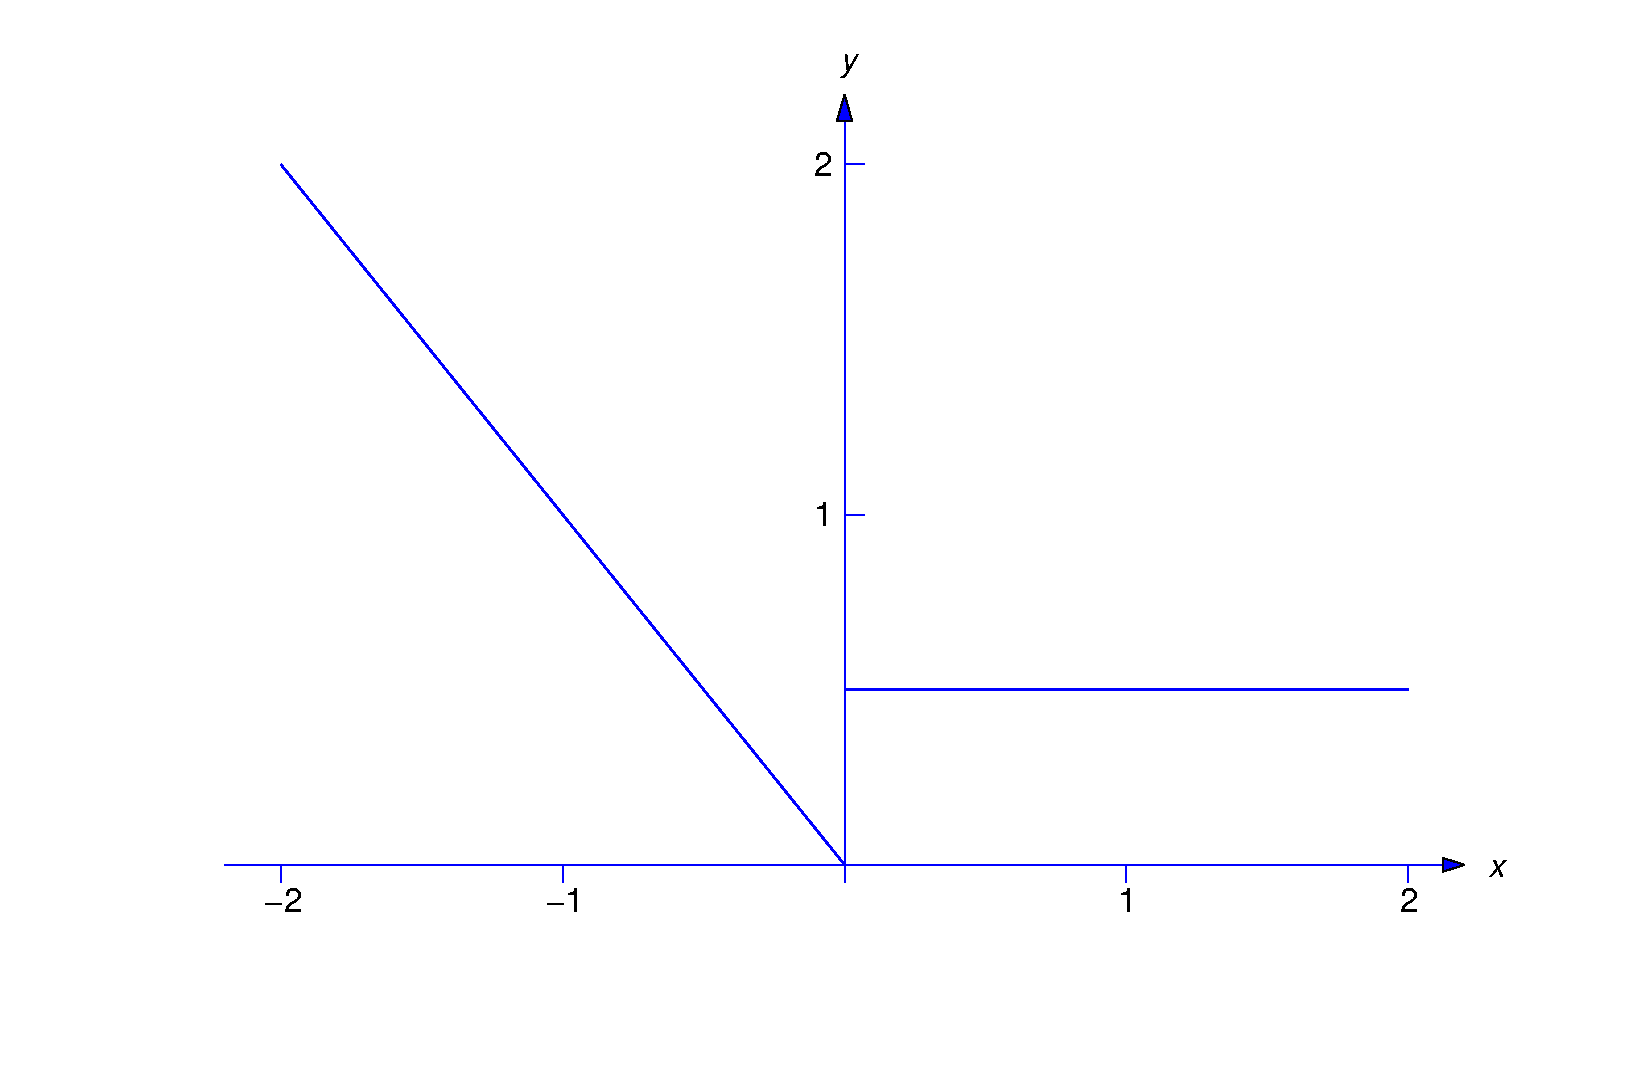
\includegraphics[bb=-78 148 689 643,width=5.67in,height=3.66in,keepaspectratio]{fig110201}
\caption{}
  \label{figure:11.2.1}
\end{figure}

\solution
Note that wen't bothered to define $f(-2)$, $f(0)$, and
$f(2)$.
 No matter
how they may be defined, $f$ is piecewise smooth on $[-2,2]$, and
the coefficients in the Fourier series
$$
F(x)=a_0+\sum_{n=1}^\infty\left(a_n\cos{n\pi
x\over2}+b_n\sin{n\pi x\over2}\right)
$$
are not affected by them. In any case,
Theorem~\ref{thmtype:11.2.4} implies that $F(x)=f(x)$ in $(-2,0)$
and $(0,2)$, where $f$ is continuous, while
$$
F(-2)=F(2)={f(-2+)+f(2-)\over2}=
{1\over2}\left(2+{1\over2}\right)={5\over4}
$$
and
$$
F(0)={f(0-)+f(0+)\over2}={1\over2}\left(0+{1\over2}\right)={1\over4}.
$$
To summarize,
$$
F(x)=
\left\{\begin{array}{rl}
{5\over4},&\phantom{-}x=-2\\[2\jot]
-x,&-2<x<0,\\[2\jot]
 {1\over4},&\phantom{-}x=0,\\[2\jot]
{1\over2},&\phantom{-}0<x<2,\\[2\jot]
{5\over4},&\phantom{-}x=2.
\end{array}\right.
$$

We compute the Fourier coefficients as follows:
$$
a_0={1\over4}\int_{-2}^2f(x)\,dx={1\over4}\left[\int_{-2}^0(-x)\,dx
+\int_0^2{1\over2}\,dx\right]
={3\over4}.
$$
If $n\ge1$, then
\begin{eqnarray*}
a_n&=&{1\over2}\int_{-2}^2f(x)\cos{n\pi
x\over2}\,dx={1\over2}\left[\int_{-2}^0(-x)\cos{n\pi x\over2}\,dx
+\int_0^2{1\over2}\cos{n\pi x\over2}\,dx\right]\\&=&{2\over
n^2\pi^2}(\cos n\pi-1),
\end{eqnarray*}
and
\begin{eqnarray*}
b_n&=&{1\over2}\int_{-2}^2f(x)\sin{n\pi
x\over2}\,dx={1\over2}\left[\int_{-2}^0(-x)\sin{n\pi x\over2}\,dx
+\int_0^2{1\over2}\sin{n\pi x\over2}\,dx\right]\\
&=&{1\over2n\pi}(1+3\cos n\pi).
\end{eqnarray*}
Therefore
$$
F(x)={3\over4}+{2\over\pi^2}\sum_{n=1}^\infty{\cos n\pi-1\over
n^2}\cos{n\pi x\over2}+{1\over2\pi}\sum_{n=1}^\infty{1+3\cos
n\pi\over n}\sin{n\pi x\over2}.
$$
Figure~\ref{figure:11.2.2} shows how the partial sum
$$
F_m(x)={3\over4}+{2\over\pi^2}\sum_{n=1}^m{\cos n\pi-1\over
n^2}\cos{n\pi x\over2}+{1\over2\pi}\sum_{n=1}^m{1+3\cos
n\pi\over n}\sin{n\pi x\over2}
$$
approximates $f(x)$ for $m=5$ (dotted curve), $m=10$  (dashed curve),
and $m=15$ (solid curve).

\begin{figure}[H]
  \centering\color{blue}
  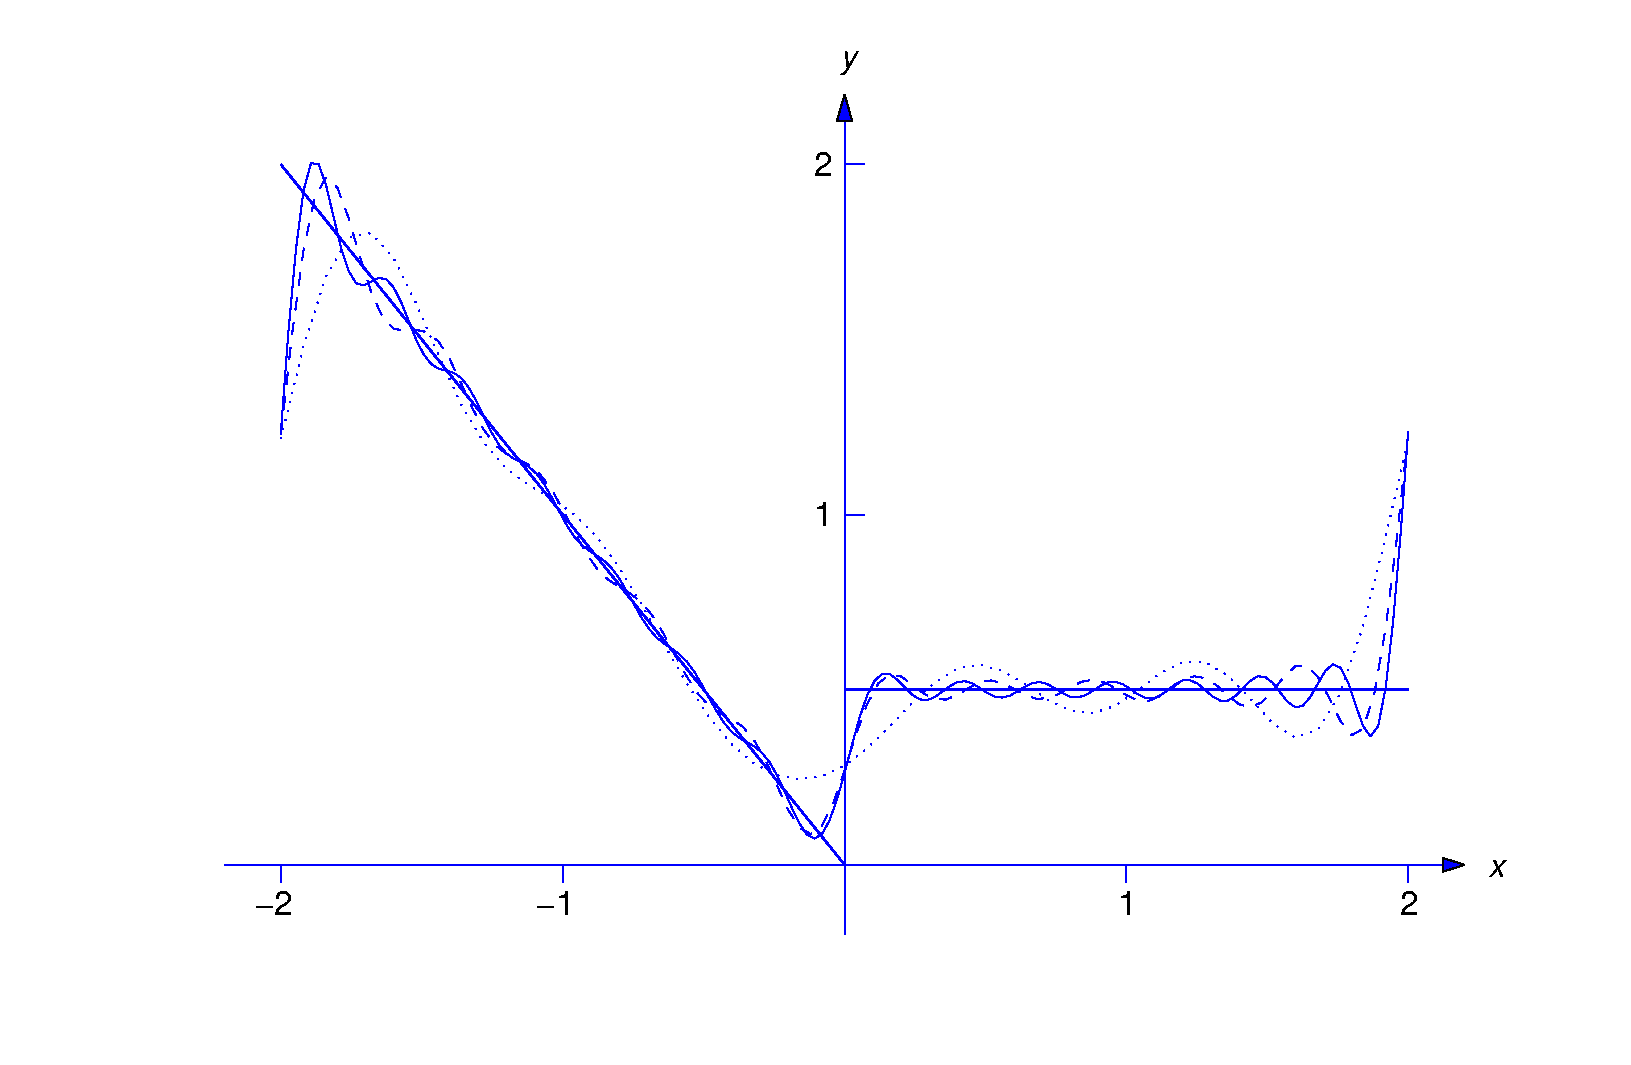
\includegraphics[bb=-78 148 689 643,width=5.67in,height=3.66in,keepaspectratio]{fig110202}
\caption{}
  \label{figure:11.2.2}
\end{figure}

\newpage
\boxit{Even and Odd Functions}

\noindent
Computing the Fourier coefficients of a  function  $f$
 can be tedious;     however,  the computation
can often be simplified by exploiting symmetries
in
$f$ or  some of its terms. To focus on this,
we recall some concepts that you studied in calculus.
Let $u$ and $v$ be defined on $[-L,L]$ and suppose
that
$$
u(-x)=u(x)\quad\mbox{ and }\quad v(-x)=-v(x),\quad -L\le x\le L.
$$
Then we say that $u$ is an {\color{blue}\it even\/} function and $v$  is an
{\color{blue}\it odd function\/}. Note that:
\begin{itemize}
\item
The product of two even functions is even.
\item
The product of two odd functions is even.
\item
The product of an even  function and an odd function  is odd.
\end{itemize}

\begin{example}\label{example:11.2.2} \rm
The functions $u(x)=\cos \omega x$ and $u(x)=x^2$  are even, while
$v(x)=\sin \omega x$ and $v(x)=x^3$ are odd. The function $w(x)=e^x$
is neither even nor odd.
\end{example}

You learned parts \part{a} and \part{b} of the  next theorem in
calculus, and the other parts follow from them
(Exercise~\ref{exer:11.2.1}).

\begin{theorem}\color{blue}\label{thmtype:11.2.5}
Suppose $u$ is even and $v$ is odd on $[-L,L].$ Then$:$
$$
\mbox{\part{a}\quad} \int_{-L}^L u(x)\,dx=2\int_0^Lu(x) \,dx,
\mbox{\quad  \part{b}\quad}
\int_{-L}^L v(x)\,dx=0,
$$
$$
\mbox{\part{c}\quad} \int_{-L}^L
u(x)\cos{n\pi x\over L}\,dx=2\int_0^Lu(x)\cos{n\pi x\over L} \,dx,
$$
$$
\mbox{\part{d}\quad}
\int_{-L}^L v(x)\sin{n\pi x\over L}\,dx=
2\int_0^L v(x)\sin{n\pi x\over L}\,dx,
$$
$$
\mbox{\part{e}\quad} \int_{-L}^L
u(x)\sin{n\pi x\over L}\,dx=0
\mbox{\quad and \quad\part{f}\quad}
\int_{-L}^L v(x)\cos{n\pi x\over L}\,dx=0.
$$
\end{theorem}

\begin{example}\label{example:11.2.3} \rm
Find the Fourier series of $f(x)=x^2-x$ on $[-2,2]$, and determine
its sum for $-2\le x\le 2$.
\end{example}

\solution Since $L=2$,
$$
F(x)=a_0+\sum_{n=1}^\infty\left(a_n\cos{n\pi
x\over2}+b_n\sin{n\pi x\over2}\right)
$$
where
\begin{equation} \label{eq:11.2.9}
a_0={1\over4}\int_{-2}^2(x^2-x)\,dx,
\end{equation}
\begin{equation} \label{eq:11.2.10}
a_n={1\over2}\int_{-2}^2(x^2-x)\cos{n\pi x\over2}\,dx,\quad
n=1,2,3,\dots,
\end{equation}
and
\begin{equation} \label{eq:11.2.11}
b_n={1\over2}\int_{-2}^2(x^2-x)\sin{n\pi x\over2}\,dx,\quad
n=1,2,3,\dots.
\end{equation}
We simplify the evaluation of these integrals by using
Theorem~\ref{thmtype:11.2.5}   with $u(x)=x^2$ and $v(x)=x$;
thus, from \eqref{eq:11.2.9},
$$
a_0={1\over2}\int_0^2x^2\,dx={x^3\over6}\lims02={4\over3}.
$$
From \eqref{eq:11.2.10},
\begin{eqnarray*}
a_n&=&\int_0^2x^2\cos{n\pi x\over2}\,dx=
{2\over n\pi}\left[x^2\sin{n\pi x\over2}\lims02-
2\int_0^2x\sin{n\pi x\over2}\,dx\right]\\
&=&{8\over n^2\pi^2}\left[x\cos{n\pi x\over2}\lims02-
\int_0^2\cos{n\pi x\over2}\,dx\right]\\
&=&{8\over n^2\pi^2}\left[2\cos n\pi-{2\over n\pi}\sin{n\pi
x\over2}\lims02\right]
=(-1)^n{16\over n^2\pi^2}.
\end{eqnarray*}
From \eqref{eq:11.2.11},
\begin{eqnarray*}
b_n&=&-\int_0^2x\sin{n\pi x\over2}\,dx
={2\over n\pi}\left[x\cos{n\pi x\over2}\lims02-
\int_0^2\cos{n\pi x\over2}\,dx\right]\\
&=&{2\over n\pi}\left[2\cos n\pi-{2\over
n\pi}\sin{n\pi x\over2}\lims02\right]=(-1)^n{4\over n\pi}.
\end{eqnarray*}
Therefore
$$
F(x)={4\over3}+{16\over\pi^2}\sum_{n=1}^\infty{(-1)^n\over n^2}
\cos{n\pi x\over2}+{4\over\pi}\sum_{n=1}^\infty
{(-1)^n\over n}\sin{n\pi x\over2}.
$$
Theorem~\ref{thmtype:11.2.4} implies that
$$
F(x)=
\left\{\begin{array}{cl}
4,&\phantom{-}x=-2,\\ x^2-x,&-2<x<2,\\4,&\phantom{-}x=2.
\end{array}\right.
$$
Figure~\ref{figure:11.2.3} shows how the partial sum
$$
F_m(x)={4\over3}+{16\over\pi^2}\sum_{n=1}^m{(-1)^n\over n^2}
\cos{n\pi x\over2}+{4\over\pi}\sum_{n=1}^m
{(-1)^n\over n}\sin{n\pi x\over2}
$$
approximates $f(x)$ for $m=5$ (dotted curve), $m=10$  (dashed curve),
and $m=15$ (solid curve).
\bbox

\begin{figure}[tbp]
  \centering\color{blue}
  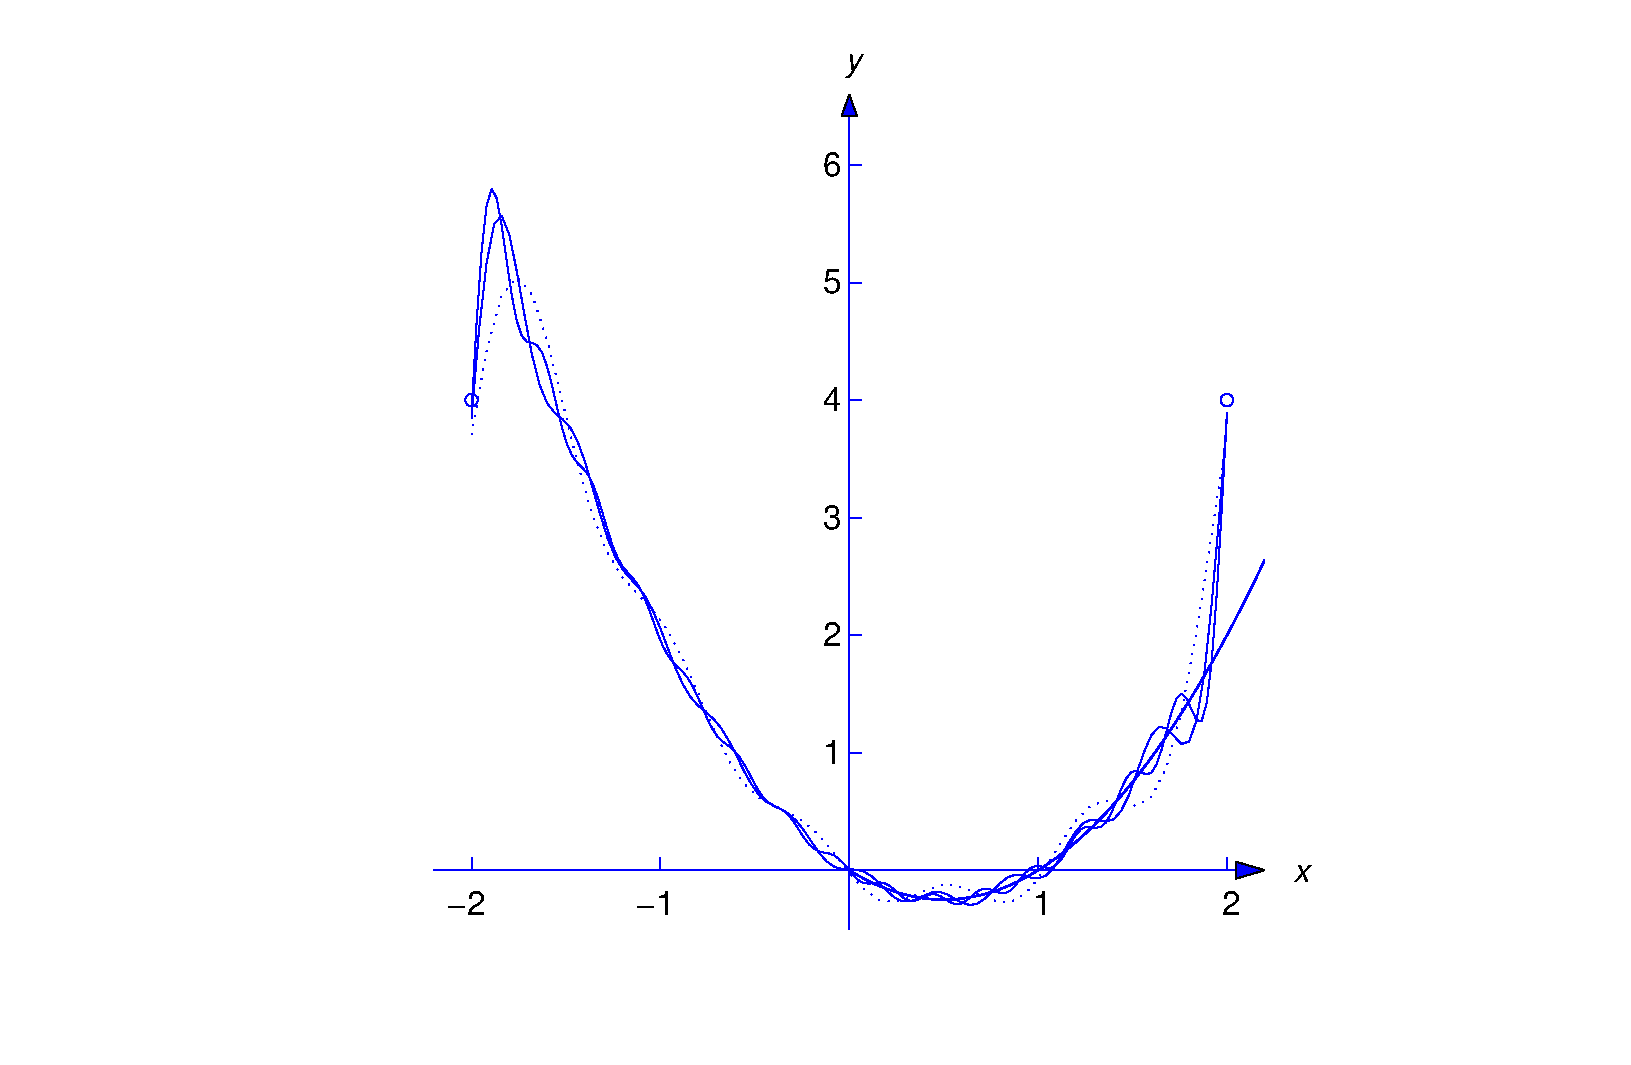
\includegraphics[bb=-78 148 689 643,width=5.67in,height=3.66in,keepaspectratio]{fig110203}
\caption{ Approximation of $f(x)=x^2-x$ by partial
sums of its Fourier series on $[-2,2]$}
  \label{figure:11.2.3}
\end{figure}

Theorem~\ref{thmtype:11.2.5} ilmplies
the next theorem follows.

\begin{theorem}\color{blue} \label{thmtype:11.2.6}
Suppose   $f$ is integrable on $[-L,L].$
\begin{alist}
\item % (a)
If $f$ is even$,$  the Fourier series of $f$ on $[-L,L]$ is
$$
F(x)=a_0+\sum_{n=1}^\infty a_n\cos{n\pi x\over L},
$$
where
$$
a_0={1\over L}\int_0^Lf(x) \,dx \mbox{\quad and \quad}
a_n={2\over L}\int_0^L f(x)\cos{n\pi x\over L}\,dx,\quad n\ge1.
$$
\item % (b)
If $f$ is odd$,$  the Fourier series of $f$ on $[-L,L]$ is
$$
F(x)= \sum_{n=1}^\infty b_n \sin{n\pi x\over L},
$$
where
$$
b_n={2\over L}\int_0^L f(x)\sin{n\pi x\over L}\,dx.
$$
\end{alist}
\end{theorem}

\begin{example}\label{example:11.2.4} \rm
Find the Fourier series of $f(x)=x$ on $[-\pi,\pi]$, and determine
its sum for $-\pi\le x\le \pi$.
\end{example}

\solution
Since $f$ is odd and $L=\pi$,
$$
F(x)=\sum_{n=1}^\infty b_n\sin nx
$$
where
\begin{eqnarray*}
b_n&=&{2\over\pi}\int_0^\pi x\sin nx\,dx=-{2\over
n\pi}\left[x\cos
nx\lims0\pi-\int_0^\pi\cos nx\,dx\right]\\
&=&-{2\over n}\cos n\pi+{2\over n^2\pi}\sin nx\lims0\pi=(-1)^{n+1}
{2\over n}.
\end{eqnarray*}
Therefore
$$
F(x)=-2\sum_{n=1}^\infty{(-1)^n\over n}\sin nx.
$$
Theorem~\ref{thmtype:11.2.4} implies that
$$
F(x)=
\left\{\begin{array}{cl}
0,&\phantom{-}x=-\pi,\\ x,&-\pi<x<\pi,\\0,&\phantom{-}x=\pi.
\end{array}\right.
$$
Figure~\ref{figure:11.2.4} shows how the partial sum
$$
F_m(x)=-2\sum_{n=1}^m{(-1)^n\over n}\sin nx
$$
approximates $f(x)$ for $m=5$ (dotted curve), $m=10$  (dashed curve),
and $m=15$ (solid curve).

\begin{figure}[tbp]
  \centering\color{blue}
  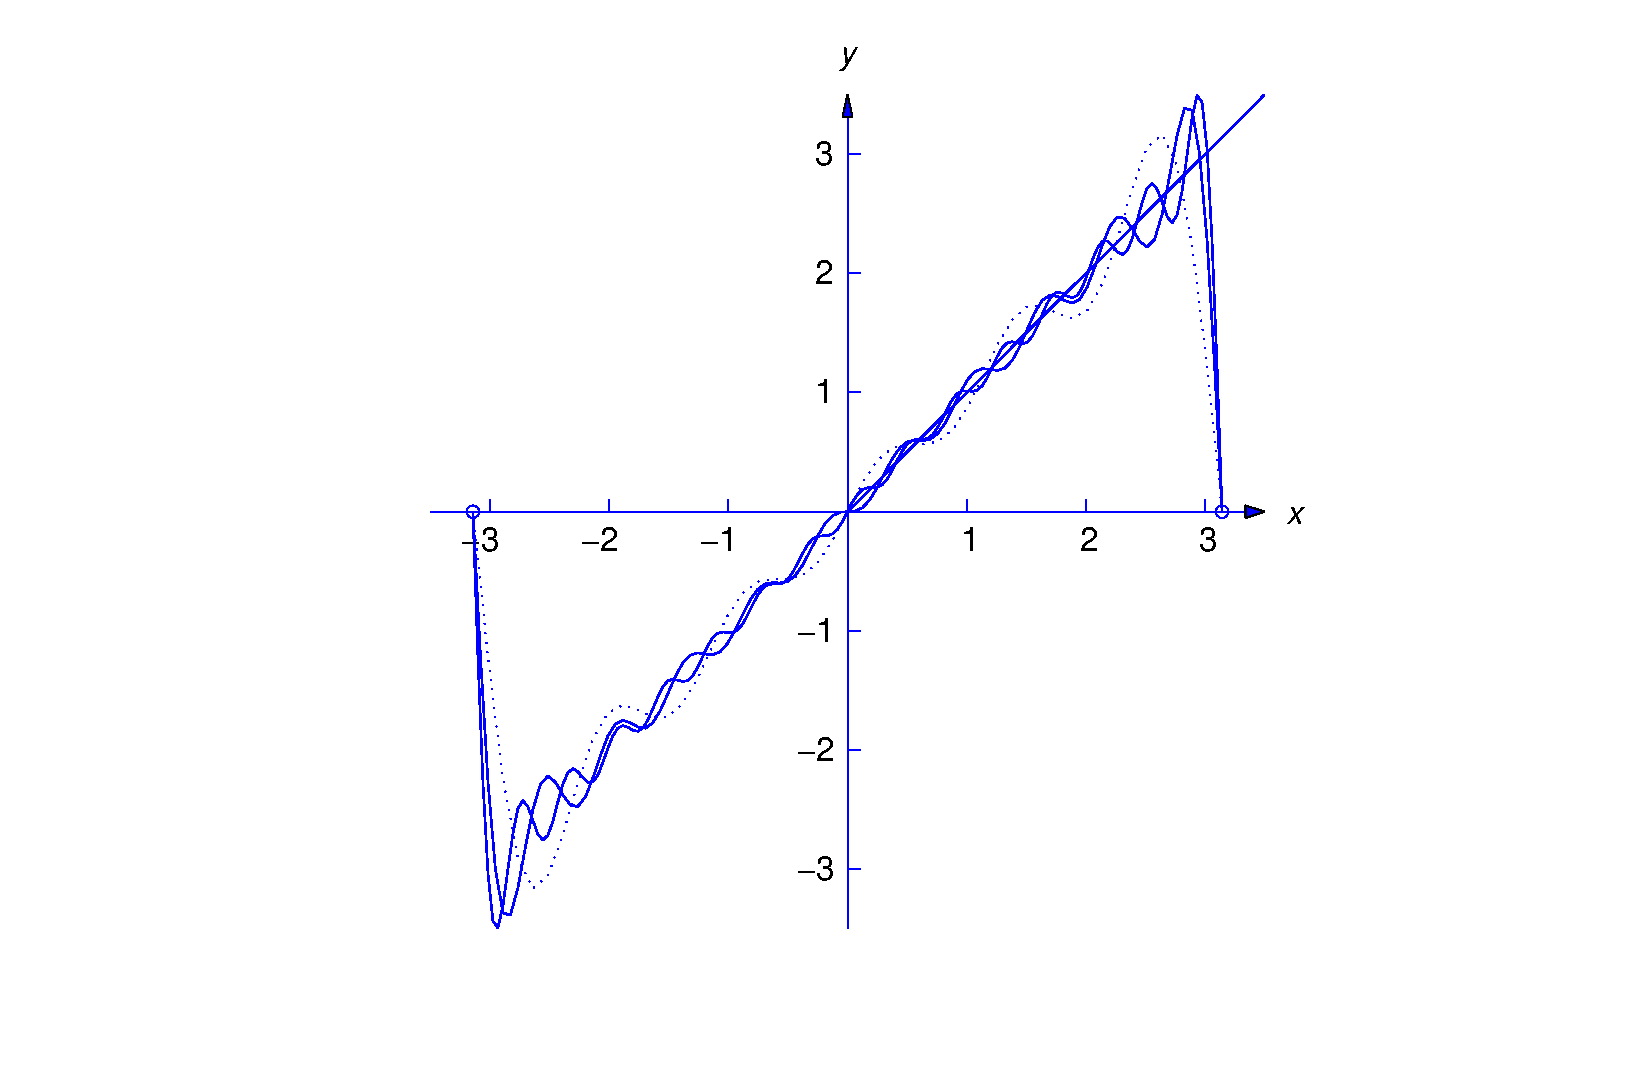
\includegraphics[bb=-78 148 689 643,width=5.67in,height=3.66in,keepaspectratio]{fig110204}
\caption{Approximation of $f(x)=x$ by partial sums
of its Fourier series on $[-\pi,\pi]$}
  \label{figure:11.2.4}
\end{figure}

\begin{example}\label{example:11.2.5} \rm
Find the Fourier series of $f(x)=|x|$ on $[-\pi,\pi]$ and
determine its sum for\\ $-\pi\le x\le\pi$.
\end{example}

\solution
Since $f$ is even and $L=\pi$,
$$
F(x)=a_0+\sum_{n=1}^\infty a_n\cos nx.
$$
Since $f(x)=x$ if $x\ge0$,
$$
a_0={1\over\pi}\int_0^\pi x\,dx={x^2\over2\pi}\lims0\pi={\pi\over2}
$$
and, if $n\ge1$,
\begin{eqnarray*}
a_n&=&{2\over\pi}\int_0^\pi x\cos nx\,dx={2\over n\pi}\left[x\sin
nx\lims0\pi-\int_0^\pi\sin nx\,dx\right]\\
&=&{2\over n^2\pi}\cos
nx\lims0\pi=\frac{2}{n^2\pi}(\cos n\pi-1)={2\over n^2\pi}[(-1)^n-1].
\end{eqnarray*}
Therefore
\begin{equation} \label{eq:11.2.12}
F(x)={\pi\over2}+{2\over\pi}\sum_{n=0}{(-1)^n-1\over n^2}\cos nx.
\end{equation}
However, since
$$
(-1)^n-1=
\left\{\begin{array}{rl} 0&\mbox{ if }n=2m,\\
-2&\mbox{ if }n=2m+1,
\end{array}\right.
$$
the terms in  \eqref{eq:11.2.12} for which $n=2m$ are all zeros.
Therefore we only to include the terms for which $n=2m+1$;
that is, we can rewrite \eqref{eq:11.2.12} as
$$
F(x)={\pi\over2}-{4\over\pi}\sum_{m=0}^\infty {1\over(2m+1)^2}
\cos(2m+1)x.
$$
However, since the name of the index of summation doesn't matter,
we prefer to replace $m$ by $n$, and write
$$
F(x)={\pi\over2}-{4\over\pi}\sum_{n=0}^\infty {1\over(2n+1)^2}
\cos(2n+1)x.
$$
Since $|x|$ is continuous for all $x$ and $|-\pi|=|\pi|$,
Theorem~\ref{thmtype:11.2.4} implies that $F(x)=|x|$ for
all $x$ in $[-\pi,\pi]$.

\begin{example}\label{example:11.2.6} \rm
Find the Fourier series of $f(x)=x(x^2-L^2)$  on $[-L,L]$,
and determine its sum for $-L\le x\le L$.
\end{example}

\solution
Since $f$ is odd,
$$
F(x)=\sum_{n=1}^\infty b_n\sin\frac{n\pi x}{L},
$$
where
\begin{eqnarray*}
b_n&=&{2\over L}\int_0^Lx(x^2-L^2)\sin{n\pi x\over L}\,dx\\
&=&-{2\over n\pi}\left[x(x^2-L^2)\cos{n\pi x\over L}\lims0L-
\int_0^L
(3x^2-L^2)\cos{n\pi x\over L}\,dx\right]\\
&=&{2L\over n^2\pi^2}\left[(3x^2-L^2)\sin{n\pi x\over
L}\lims0L-6
\int_0^Lx\sin{n\pi x\over L}\,dx\right]\\
&=&{12L^2\over n^3\pi^3}\left[x\cos{n\pi x\over L}\lims0L-
\int_0^L\cos{n\pi x\over L}\,dx\right]
=(-1)^n{12L^3\over n^3\pi^3}.
\end{eqnarray*}
Therefore
$$
F(x)={12L^3\over\pi^3}\sum_{n=1}^\infty{(-1)^n\over n^3}\sin{n\pi
x\over L}.
$$
Theorem~\ref{thmtype:11.2.4} implies that $F(x)=x(x^2-L^2)$ for all $x$
in $[-L,L]$.

\begin{example}[Gibbs Phenomenon]\label{example:11.2.7}\rm
The Fourier series of
$$
f(x)=\left\{\begin{array}{cl}
0,&-1<x<-{1\over2},\\
1,&-{1\over2}<x<{1\over2},\\[2\jot]
0,&\phantom{-}{1\over2}<x<1
\end{array}\right.
$$
on $[-1,1]$ is
$$
F(x)={1\over2}+{2\over\pi}\sum_{n=1}^\infty
{(-1)^{n-1}\over2n-1}\cos(2n-1)\pi x.
$$
(Verify.) According to Theorem~\ref{thmtype:11.2.4},
$$
F(x)=\left\{\begin{array}{cl}
0,&-1\le x<-{1\over2},\\
{1\over2},& x=-{1\over2},\\
1,&-{1\over2}<x<{1\over2},\\
{1\over2},& x={1\over2},\\
0,&{1\over2}<x\le 1;
\end{array}\right.
$$
thus, $F$ (as well as $f$) has unit jump discontinuities
at $x=\pm\frac{1}{2}$.
Figures~\ref{figure:11.2.5}-\ref{figure:11.2.7} show the graphs
of $y=f(x)$ and
$$
y=F_{2N-1}(x)=\frac{1}{2}+
{2\over\pi}\sum_{n=1}^N {(-1)^{n-1}\over2n-1}\cos(2n-1)\pi x
$$
for $N=10$, $20$, and $30$. You can see that although $F_{2N-1}$
approximates $F$ (and therefore $f$) well on larger intervals as $N$
increases, the maximum absolute values of the errors
remain approximately equal to $.09$, but occur closer to the
discontinuities $x=\pm\frac{1}{2}$ as $N$ increases.
\end{example}

\begin{figure}[H]
\color{blue}
  \begin{minipage}[b]{0.5\linewidth}
    \centering
   \scalebox{.65}{
  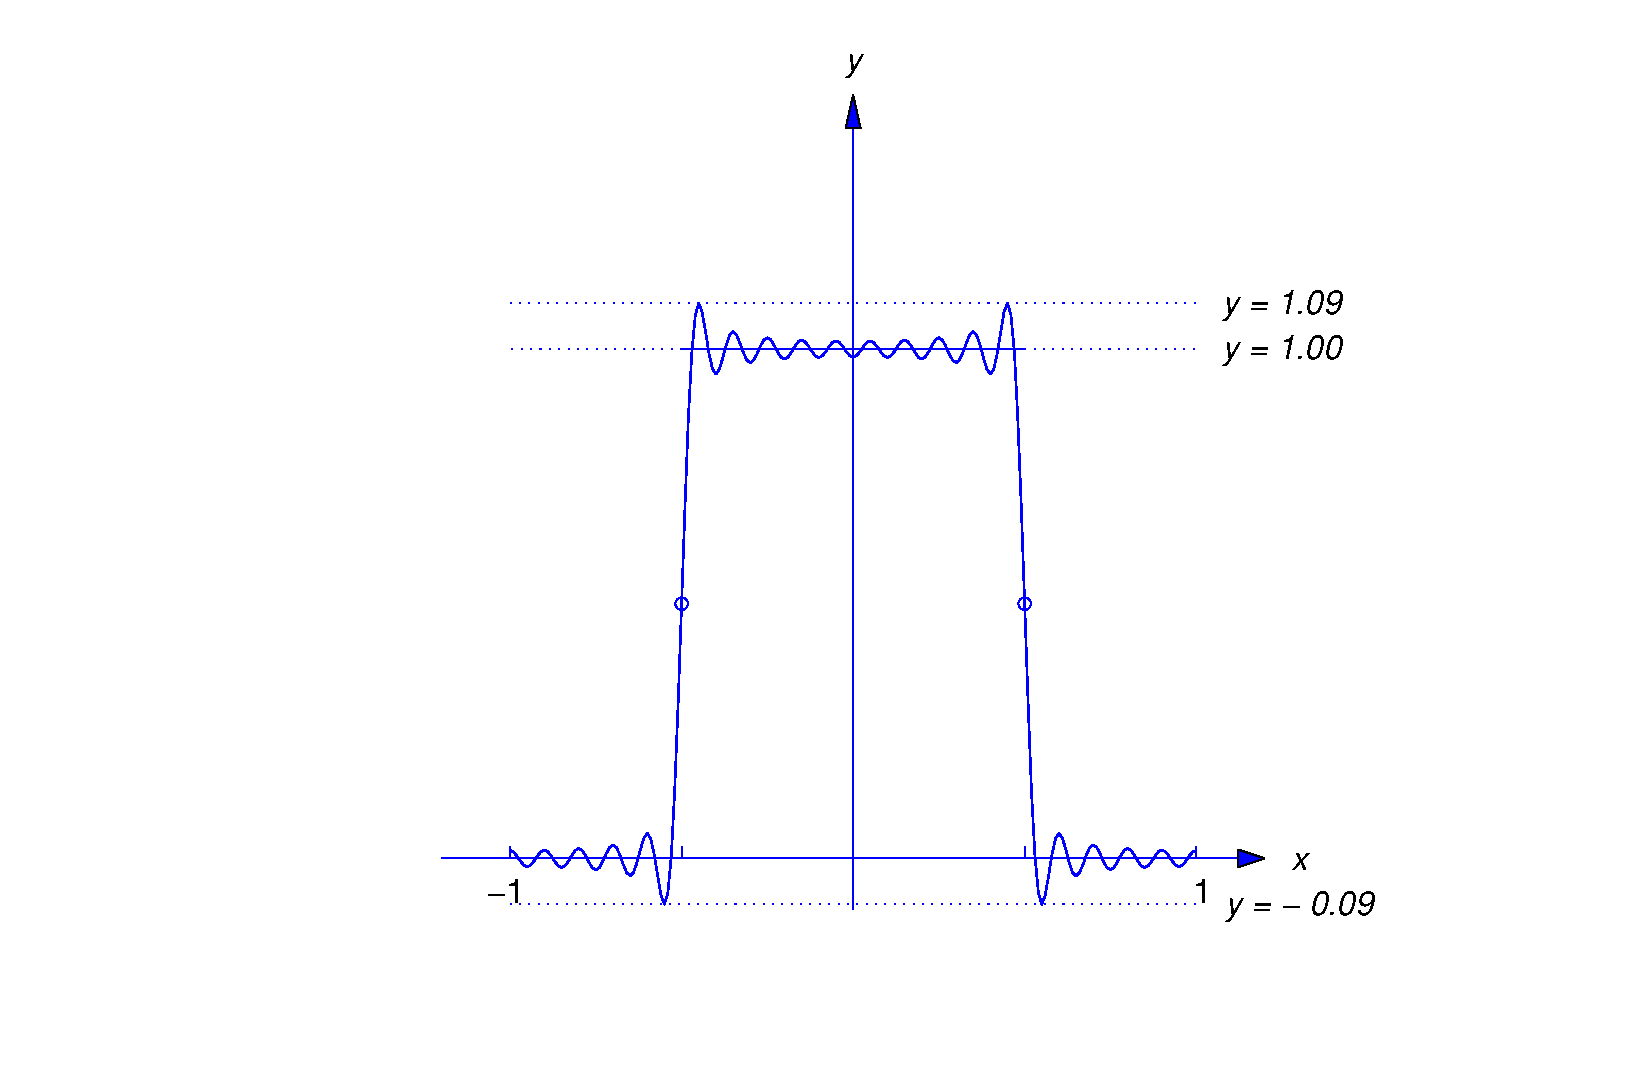
\includegraphics[bb=-78 148 689 643,width=5.67in,height=3.66in,keepaspectratio]{fig110205}}
\caption{ The Gibbs Phenomenon:
Example~\ref{example:11.2.7}, $N=10$}
  \label{figure:11.2.5}
\end{minipage}
  \begin{minipage}[b]{0.5\linewidth}
    \centering
   \scalebox{.65}{
  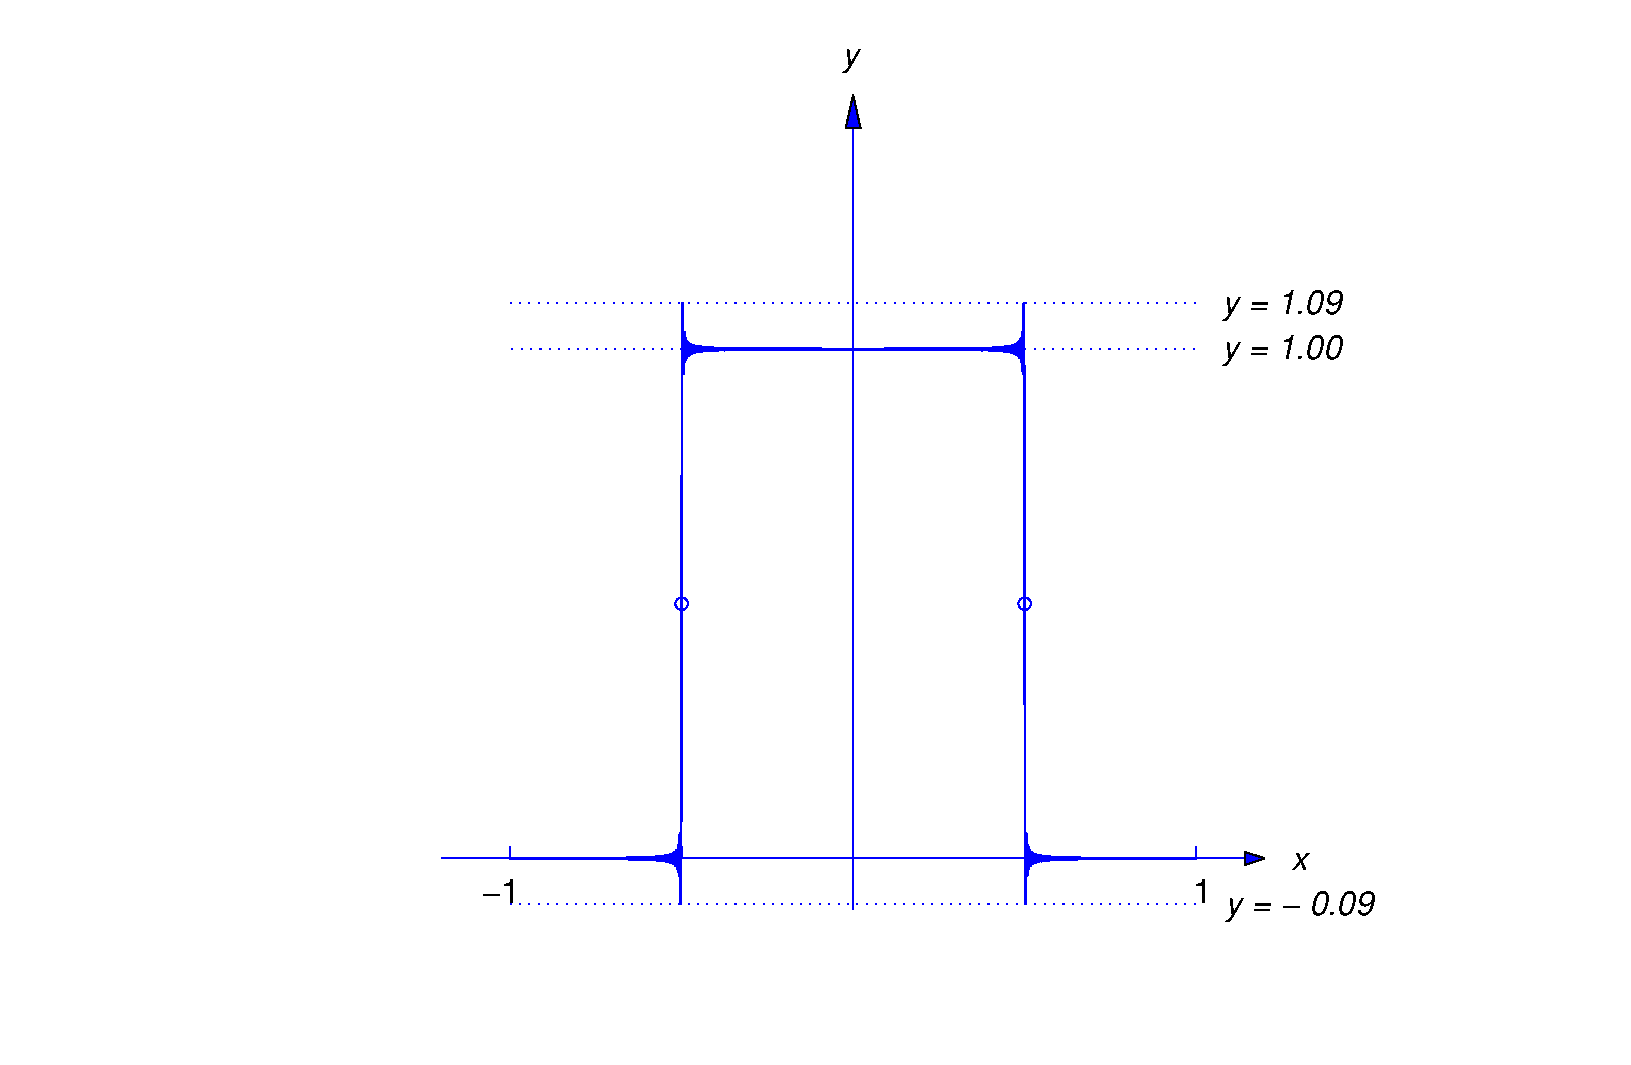
\includegraphics[bb=-78 148 689 643,width=5.67in,height=3.66in,keepaspectratio]{fig110206}}
\caption{ The Gibbs Phenomenon:
Example~\ref{example:11.2.7}, $N=20$}
  \label{figure:11.2.6}
\end{minipage}
\end{figure}

\newpage

\begin{figure}[H]
  \centering
  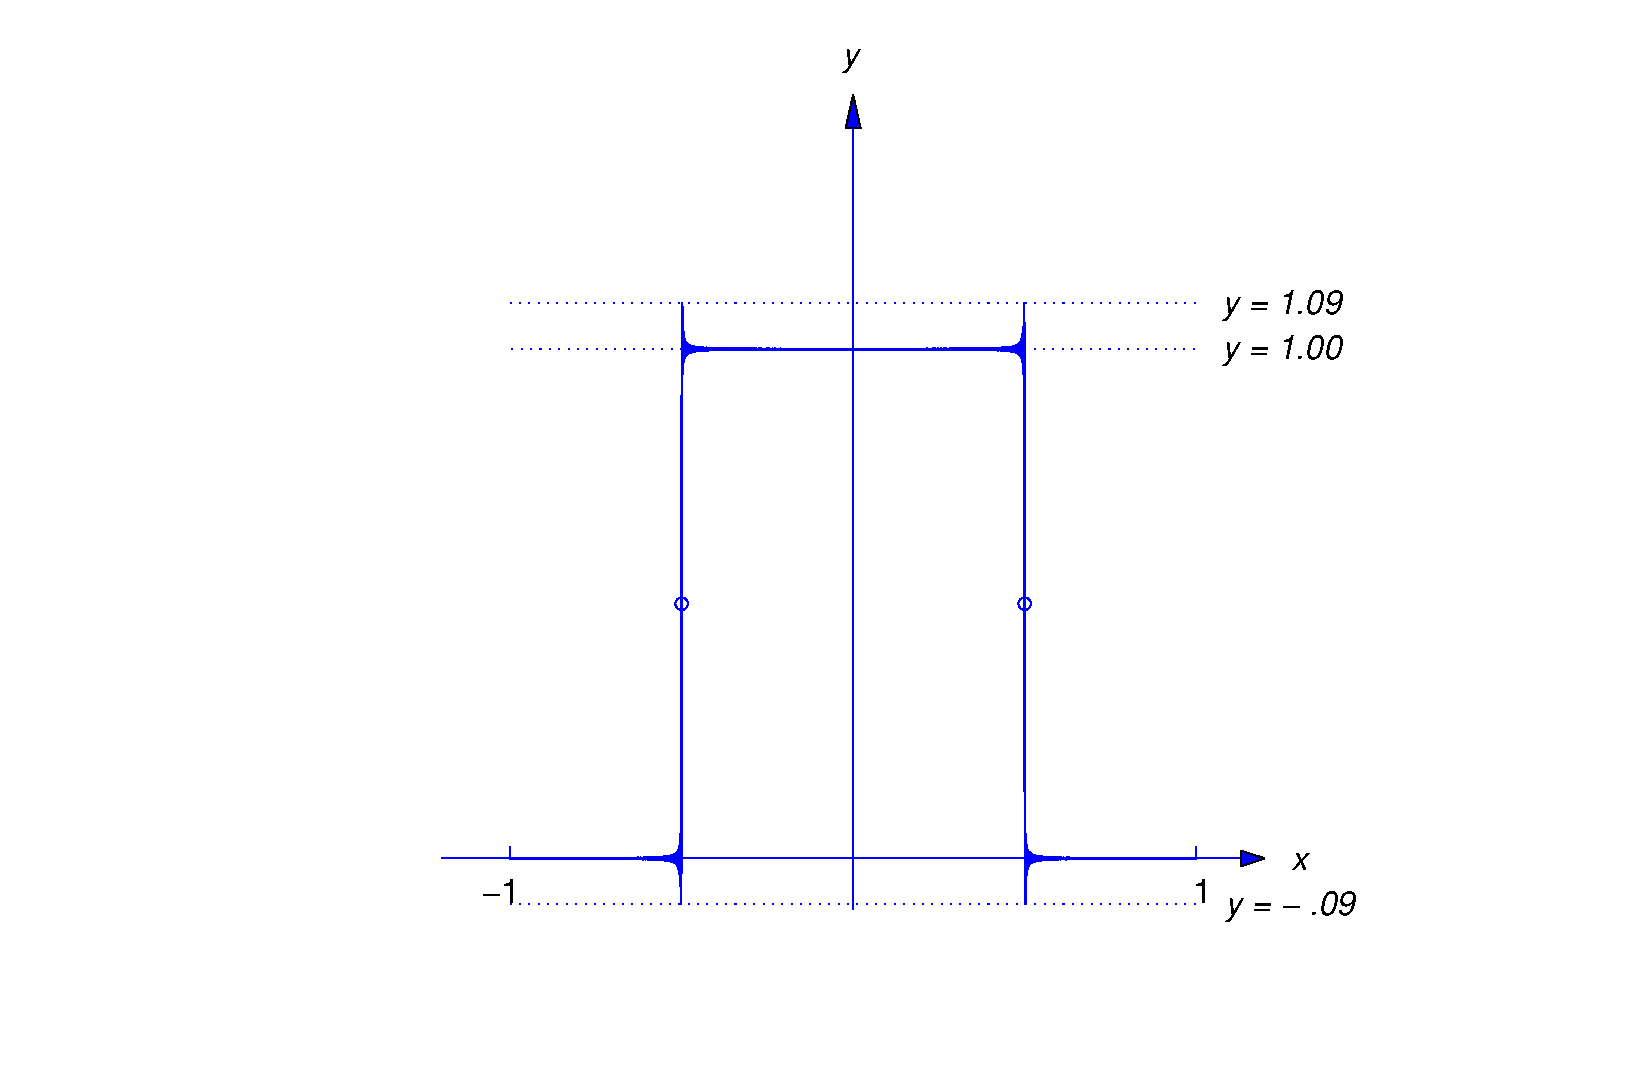
\includegraphics[bb=-78 148 689 643,width=5.67in,height=3.66in,keepaspectratio]{fig110207}
\caption{ The Gibbs Phenomenon:
Example~\ref{example:11.2.7}, $N=30$}
  \label{figure:11.2.7}
\end{figure}

\technology
\medskip

The computation of Fourier coefficients will be tedious in many of the
exercises in this chapter and the next. To learn the technique, we
recommend that you do some exercises in each section ``by hand,''
perhaps using the table of integrals at the front of the book.
However, we encourage you to use your favorite symbolic computation
software in the more difficult problems.

\exercises

\begin{exerciselist}

\item\label{exer:11.2.1}
Prove Theorem~\ref{thmtype:11.1.5}.

\exercisetext{
In Exercises~\ref{exer:11.2.2}-\ref{exer:11.2.16} find the Fourier
series of $f$ on  $[-L,L]$ and determine its sum for $-L\le x\le L$.
Where indicated by \Cex,
 graph $f$ and
$$
F_m(x)=a_0+\sum_{n=1}^m\left(a_n\cos{n\pi x\over
L}+b_n\sin{n\pi x\over L}\right)
$$
on the same axes for various values of $m$.}

\item\label{exer:11.2.2} \Cex
$L=1$;  \quad $f(x)=2-x$

\item\label{exer:11.2.3}
$L=\pi$;  \quad$f(x)=2x-3x^2$

\item\label{exer:11.2.4}
$L=1$;  \quad$f(x)=1-3x^2$

\item\label{exer:11.2.5}
$L=\pi$;  \quad$f(x)=|\sin x|$

\item\label{exer:11.2.6}  \Cex
$L=\pi$;  \quad$f(x)=x\cos x$

\item\label{exer:11.2.7}
$L=\pi$;  \quad$f(x)=|x|\cos x$

\item\label{exer:11.2.8} \Cex
$L=\pi$;  \quad$f(x)=x\sin x$

\item\label{exer:11.2.9}
$L=\pi$;  \quad$f(x)=|x|\sin x$

\item\label{exer:11.2.10}
$L=1$;  \quad$f(x)=
\left\{\begin{array}{cl}
0,&-1<x<{1\over2},\\[2\jot]
\cos\pi x,&-{1\over2}<x<{1\over2},\\[2\jot]
0,&\phantom{-}{1\over2}<x<1
\end{array}\right.$

\item\label{exer:11.2.11}
$L=1$;  \quad$f(x)=
\left\{\begin{array}{cl}
0,&-1<x<{1\over2},\\[2\jot]
x\cos\pi x,&-{1\over2}<x<{1\over2},\\[2\jot]
0,&\phantom{-}{1\over2}<x<1
\end{array}\right.$

\item\label{exer:11.2.12}
$L=1$;  \quad$f(x)=
\left\{\begin{array}{cl}
0,&-1<x<{1\over2},\\[2\jot]
\sin\pi x,&-{1\over2}<x<{1\over2},\\[2\jot]
0,&\phantom{-}{1\over2}<x<1
\end{array}\right.$

\item\label{exer:11.2.13}
$L=1$;  \quad$f(x)=
\left\{\begin{array}{cl}
0,&-1<x<{1\over2},\\[2\jot]
|\sin\pi x|,&-{1\over2}<x<{1\over2},\\[2\jot]
0,&\phantom{-}{1\over2}<x<1
\end{array}\right.$

\item\label{exer:11.2.14}
$L=1$;  \quad$f(x)=
\left\{\begin{array}{cl}
0,&-1<x<{1\over2},\\[2\jot]
x\sin\pi x,&-{1\over2}<x<{1\over2},\\[2\jot]
0,&\phantom{-}{1\over2}<x<1
\end{array}\right.$

\item\label{exer:11.2.15} \Cex
$L=4$;  \quad
$f(x)=
\left\{\begin{array}{cl}
0,&-4<x<0,\\x,&\phantom{-}0<x<4
\end{array}\right.$

\item\label{exer:11.2.16} \Cex
$L=1$;  \quad $f(x)=
\left\{\begin{array}{cl}
x^2,&-1< x<0,
\\1-x^2,&\phantom{-}0<x<1
\end{array}\right.$

\item\label{exer:11.2.17} \Lex Verify the Gibbs phenomenon for
\quad $f(x)=
\left\{\begin{array}{rl}
2,&-2< x<
-1,\\1,&-1<x<1,\\-1,&\phantom{-}1< x<2.
\end{array}\right.$

\item\label{exer:11.2.18} \Lex Verify the Gibbs phenomenon for
\quad $f(x)=
\left\{\begin{array}{rl}
2,&-3< x<
-2,\\3,&-2<x<2,\\1,&\phantom{-}2< x<3.
\end{array}\right.$

\item\label{exer:11.2.19}
Deduce from  Example~\ref{example:11.2.5} that
$$
\sum_{n=0}^\infty{1\over(2n+1)^2}={\pi^2\over 8}.
$$

\item\label{exer:11.2.20}
\begin{alist}
\item % (a)
Find the Fourier series of $f(x)=e^x$ on $[-\pi,\pi]$.
\item % (b)
Deduce from  \part{a}  that
$$
\sum_{n=0}^\infty{1\over n^2+1}={\pi\coth\pi-1\over2}.
$$
 \end{alist}

\item\label{exer:11.2.21}
Find the Fourier series of $f(x)=(x-\pi)\cos x$ on $[-\pi,\pi]$.

\item\label{exer:11.2.22}
Find the Fourier series of $f(x)=(x-\pi)\sin x$ on $[-\pi,\pi]$.

\item\label{exer:11.2.23}
Find the Fourier series  of $f(x)=\sin kx$ ($k\ne$
integer) on $[-\pi,\pi]$.

\item\label{exer:11.2.24}
Find the Fourier series  of $f(x)=\cos kx$ ($k\ne$
integer) on $[-\pi,\pi]$.

\item\label{exer:11.2.25}
\begin{alist}
\item % (a)
Suppose $g'$ is continuous on $[a,b]$ and $\omega\ne0$.
Use integration by parts to show that there's a constant $M$ such
that
$$
\left|\int_a^bg(x)\cos\omega x\,dx\right|\le{M\over\omega}
\mbox{\quad and \quad}
\left|\int_a^bg(x)\sin\omega x\,dx\right|\le{M\over\omega},\quad
\omega>0.
$$
\item % (b)
Show that the conclusion of \part{a} also holds if $g$
is piecewise smooth on $[a,b]$.  (This is a special case
of
\href{http://www-history.mcs.st-and.ac.uk/Mathematicians/Riemann.html}
{\color{blue}\it Riemann's Lemma}.
\item % (c)
We say that a sequence $\{\alpha_n\}_{n=1}^\infty$  is {\color{blue}\it of
order $n^{-k}$\/} and write
$\alpha_n=O(1/n^k)$
if  there's a constant $M$ such that
$$
|\alpha_n|<{M\over n^k},\quad n=1,2,3,\dots.
$$
Let $\{a_n\}_{n=1}^\infty$ and $\{b_n\}_{n=1}^\infty$
be the Fourier coefficients of a piecewise smooth function.
Conclude from \part{b} that $a_n=O(1/n)$  and $b_n=O(1/n)$.
\end{alist}

\item\label{exer:11.2.26}
\begin{alist}
\item % (a)
Suppose $f(-L)=f(L)$, $f'(-L)=f'(L)$,  $f'$ is continuous,
and $f''$ is piecewise continuous
on $[-L,L]$.
Use Theorem~\ref{thmtype:11.2.4} and integration by parts to show that
$$
f(x)=a_0+\sum_{n=1}^\infty\left(a_n\cos{n\pi x\over L}+b_n\sin{n\pi
x\over L}\right),\quad -L\le x\le L,
$$
with
$$
a_0={1\over 2L}\int_{-L}^L f(x)\,dx,
$$
$$
a_n= -{L\over n^2\pi^2}\int_{-L}^L f''(x)\cos{n\pi
x\over L}\,dx,\mbox{\quad and \quad}
b_n=-{L\over n^2\pi^2}\int_{-L}^L f''(x)\sin{n\pi x\over
L}\,dx,\,n\ge1.
$$
\item % (b)
Show that if, in addition to the  assumptions in \part{a},  $f''$ is
continuous and $f'''$ is piecewise continuous on
$[-L,L]$, then
$$
a_n={L^2\over n^3\pi^3}\int_{-L}^Lf'''(x)\sin{n\pi x\over L}\,dx.
$$
\end{alist}

\item\label{exer:11.2.27}
Show that if $f$ is integrable on $[-L,L]$ and
$$
f(x+L)=f(x),\quad -L<x<0
$$
(Figure~\ref{figure:11.2.8}), then the Fourier series of $f$ on $[-L,L]$
has the form
$$
A_0+\sum_{n=1}^\infty\left(A_n\cos{2n\pi\over
L}+B_n\sin{2n\pi\over L}\right)
$$
where
$$
A_0={1\over L}\int_0^Lf(x)\,dx,
$$
and
$$
A_n={2\over L}\int_0^Lf(x)\cos{2n\pi x\over L}\,dx, \quad
B_n={2\over L}\int_0^Lf(x)\sin{2n\pi x\over L}\,dx,\quad
n=1,2,3,\dots.
$$

\begin{figure}[H]
\color{blue}
  \begin{minipage}[b]{0.5\linewidth}
    \centering
   \scalebox{.65}{
  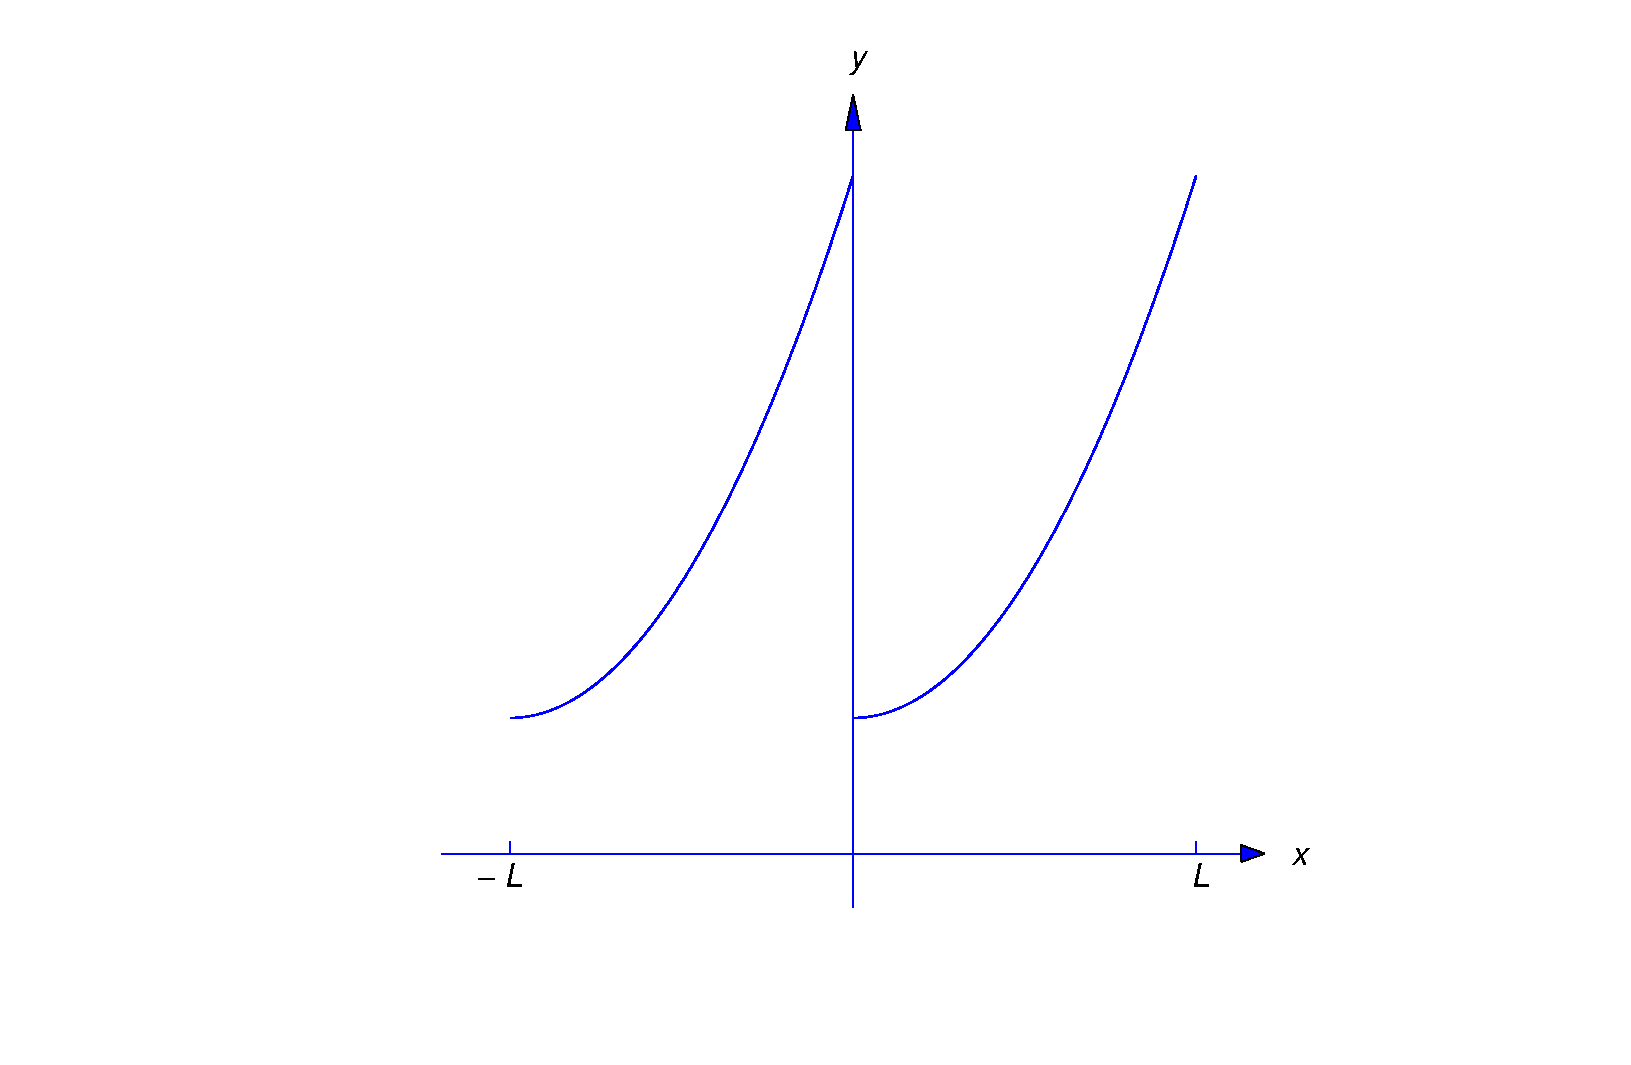
\includegraphics[bb=-78 148 689 643,width=5.67in,height=3.66in,keepaspectratio]{fig110208}}
\caption{ $y=f(x)$, where $f(x+L)=f(x)$,\, $-L<x<0$}
  \label{figure:11.2.8}
\end{minipage}
  \begin{minipage}[b]{0.5\linewidth}
    \centering
   \scalebox{.65}{
  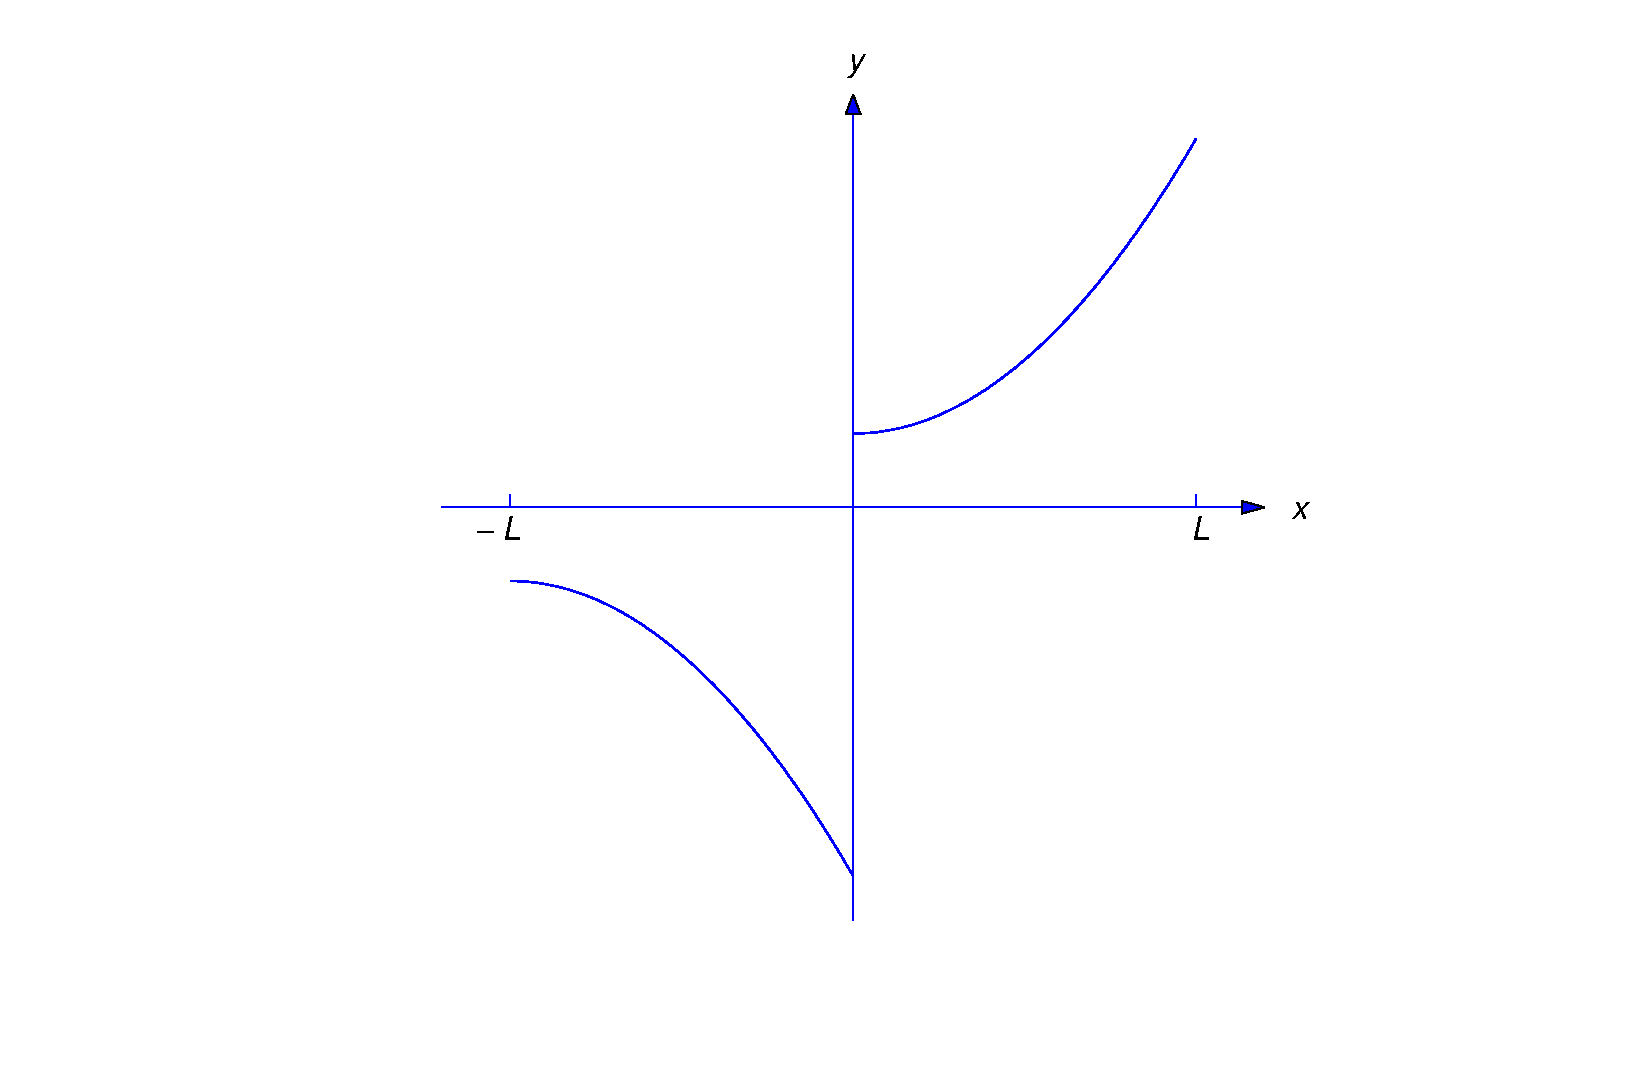
\includegraphics[bb=-78 148 689 643,width=5.67in,height=3.66in,keepaspectratio]{fig110209}}
\caption{ $y=f(x)$, where $f(x+L)=-f(x)$,
$-L<x<0$}
  \label{figure:11.2.9}
\end{minipage}
\end{figure}

\item\label{exer:11.2.28}
Show that if $f$ is integrable on $[-L,L]$ and
$$
f(x+L)=-f(x),\quad -L<x<0
$$
(Figure~\ref{figure:11.2.9}), then the Fourier series of $f$ on $[-L,L]$
has the form
$$
\sum_{n=1}^\infty\left(A_n\cos{(2n-1)\pi x\over
L}+B_n\sin{(2n-1)\pi x\over L}\right),
$$
where
$$
A_n={2\over L}\int_0^Lf(x)\cos{(2n-1)\pi x\over L}\,dx
\text{\quad and \quad }
B_n={2\over L}\int_0^Lf(x)\sin{(2n-1)\pi x\over L}\,dx,\quad
n=1,2,3,\dots.
$$

\item\label{exer:11.2.29}
Suppose $\phi_1$, $\phi_2$, \dots, $\phi_m$ are orthogonal
on $[a,b]$ and
$$
\int_a^b\phi_n^2(x)\,dx\ne0,\quad n=1,2,\dots,m.
$$
If $a_1$, $a_2$, \dots, $a_m$ are arbitrary real numbers,
define
$$
P_m=a_1\phi_1+a_2\phi_2+\cdots+a_m\phi_m.
$$
Let
$$
F_m=c_1\phi_1+c_2\phi_2+\cdots+c_m\phi_m,
$$
where
$$
c_n={\int_a^bf(x)\phi_n(x)\,dx\over\int_a^b\phi_n^2(x)\,dx};
$$
that is, $c_1$, $c_2$, \dots, $c_m$ are   Fourier coefficients of
$f$.
\begin{alist}
\item % (a)
Show that
$$
\int_a^b(f(x)-F_m(x))\phi_n(x)\,dx=0,\quad n=1,2,\dots,m.
$$
\item % (b)
Show that
$$
\int_a^b(f(x)-F_m(x))^2\,dx\le
\int_a^b(f(x)-P_m(x))^2\,dx,
$$
with equality if and only if $a_n=c_n$, $n=1,2,\dots, m$.
\item % (c)
Show that
$$
\int_a^b(f(x)-F_m(x))^2\,dx=\int_a^bf^2(x)\,dx-\sum_{n=1}^mc_n^2\int_a^b
\phi_n^2\,dx.
$$
\item % (d)
Conclude from \part{c} that
$$
\sum_{n=1}^m c_n^2\int_a^b\phi_n^2(x)\,dx\le \int_a^bf^2(x)\,dx.
$$
\end{alist}

\item\label{exer:11.2.30}
If $A_0$, $A_1$, \dots, $A_m$ and $B_1$, $B_2$, \dots, $B_m$
are arbitrary constants we say that
$$
P_m(x)=A_0+\sum_{n=1}^m\left(A_n\cos{n\pi x\over L}+B_n\sin{n\pi x\over L}\right)
$$
is a {\color{blue}\it trigonometric polynomial of degree $\le m$\/}.

Now let
$$
a_0+\sum_{n=1}^\infty\left(a_n\cos{n\pi x\over L}+b_n\sin{n\pi x\over L}\right)
$$
be the Fourier series of an integrable function $f$ on $[-L,L]$,
and let
$$
F_m(x)=
a_0+\sum_{n=1}^m\left(a_n\cos{n\pi x\over L}+b_n\sin{n\pi x\over L}\right).
$$
\begin{alist}
\item % (a)
Conclude from Exercise~\ref{exer:11.2.29}\part{b} that
$$
\int_{-L}^L(f(x)-F_m(x))^2\,dx\le
\int_{-L}^L(f(x)-P_m(x))^2\,dx,
$$
with equality if and only if $A_n=a_n$, $n=0$, $1$, \dots, $m$, and
$B_n=b_n$, $n=1$, $2$, \dots, $m$.
\item % (b)
Conclude from Exercise~\ref{exer:11.2.29}\part{d} that
$$
2a_0^2+\sum_{n=1}^m(a_n^2+b_n^2)\le{1\over L}\int_{-L}^Lf^2(x)\,dx
$$
for every $m\ge0$.
\item % (c)
Conclude from \part{b}  that
$\lim_{n\to\infty}a_n=\lim_{n\to\infty}b_n=0$.
\end{alist}

\end{exerciselist}


\section{Fourier Expansions II}

\noindent
In this section we discuss Fourier expansions in terms of the
eigenfunctions of Problems~1-4 for Section~{\color{red}11.1}.

\boxit{Fourier Cosine Series}

\noindent
From  Exercise~11.1.~\hspace*{-3pt}\ref{exer:11.1.20}, the eigenfunctions
$$
1,\, \cos{\pi x\over L},
\, \cos{2\pi x\over L},\dots,
 \, \cos{n\pi x\over L},\dots
$$
 of the boundary value problem
\begin{equation} \label{eq:11.3.1}
y''+\lambda y=0,\quad y'(0)=0,\quad y'(L)=0
\end{equation}
(Problem~2)  are orthogonal on $[0,L]$.
 If $f $ is integrable on $[0,L]$ then the
Fourier expansion of $f$ in terms of these functions is called the
{\color{blue}\it Fourier cosine series of $f$ on $[0,L]$\/}. This series is
$$
a_0+\sum_{n=1}^\infty a_n\cos{n\pi x\over L},
$$
where
$$
a_0={\dst\int_0^Lf(x)\,dx\over\dst\int_0^L\,dx}={1\over
L}\int_0^Lf(x)\,dx
$$
and
$$
a_n={\dst\int_0^Lf(x)\cos{n\pi x\over L}\,dx\over\dst\int_0^L
\cos^2{n\pi x\over L}\,dx}={2\over L}\int_0^Lf(x)\cos{n\pi x\over
L}\,dx,\quad n=1,2,3,\dots.
$$
Comparing this definition with
Theorem~\ref{exer:11.2.6}\part{a} shows that the Fourier cosine
series of $f$ on $[0,L]$ is  the Fourier series of
 the  function
$$
f_1(x)=
\left\{\begin{array}{cl}
f(-x),&-L<x<0,\\f(x),&\phantom{-}0\le x\le L,
\end{array}\right.
$$
obtained by extending  $f$ over $[-L,L]$ as an even
function (Figure~\ref{figure:11.3.1}).

\begin{figure}[tbp]
  \centering\color{blue}
  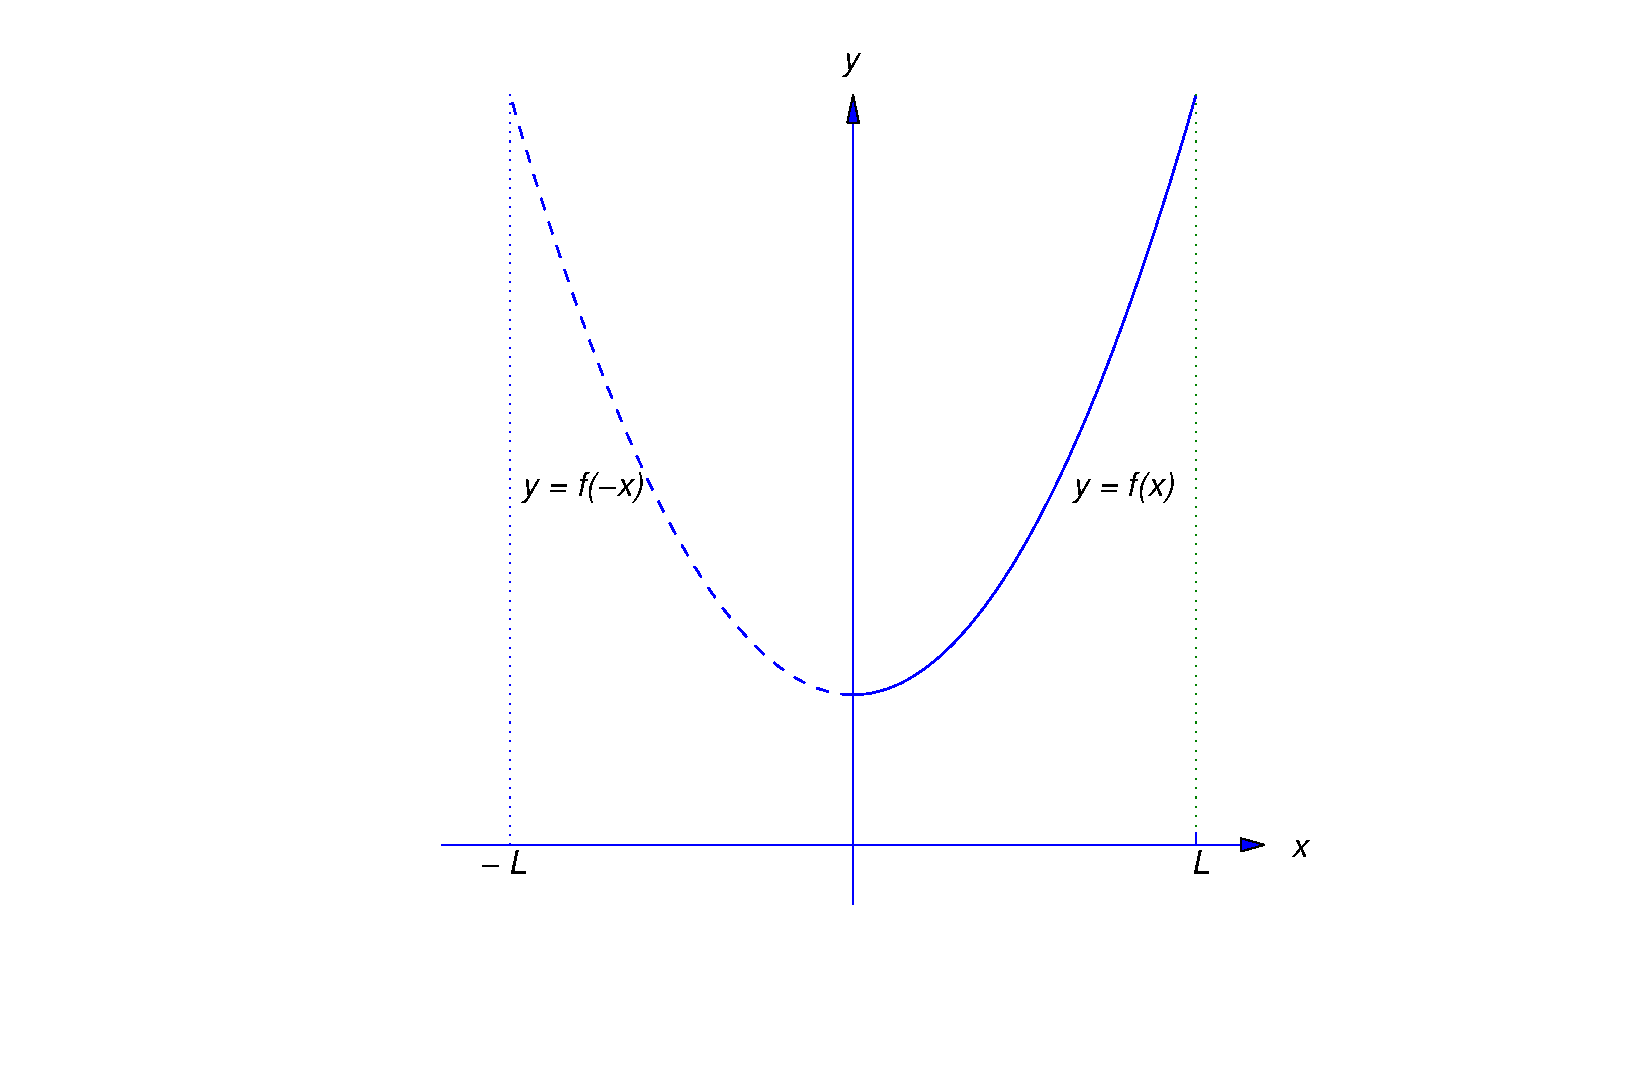
\includegraphics[bb=-78 148 689 643,width=5.67in,height=3.66in,keepaspectratio]{fig110301}
  \caption{}
  \label{figure:11.3.1}
\end{figure}

Applying
Theorem~\ref{thmtype:11.2.4} to $f_1$ yields the next
theorem.

\begin{theorem}\color{blue} \label{thmtype:11.3.1}
If $f$ is piecewise smooth on $[0,L]$, then the Fourier cosine series
$$
C(x)=a_0+\sum_{n=1}^\infty a_n\cos{n\pi x\over L}
$$
of $f$
on $[0,L]$,
with
$$
a_0={1\over L}\int_0^Lf(x)\,dx
\mbox{\quad and \quad}
a_n={2\over L}\int_0^Lf(x)\cos{n\pi x\over L}\,dx,\quad n=1,2,3,\dots,
$$
 converges for all $x$ in $[0,L]$;     moreover,
$$
C(x)=
\left\{\begin{array}{cl}
f(0+)&\mbox{if }x=0  \\
f(x)&\mbox{if $0<x<L$ and $f$ is continuous at $x  $}\\[2\jot]
\dst{f(x-)+f(x+)\over2}&\mbox{if $0<x<L$ and $f$ is discontinuous at
$x  $}\\[2\jot]
f(L-)&\mbox{if }x=L.
\end{array}\right.
$$
\end{theorem}

\begin{example}\label{example:11.3.1} \rm
Find the Fourier cosine series of $f(x)=x$ on $[0,L]$.
\end{example}

\solution
 The coefficients are
$$
a_0={1\over L}\int_0^Lx\,dx={1\over
L}{x^2\over2}
\lims0L={L\over2}
$$
and, if $n\ge1$
\begin{eqnarray*}
a_n&=&{2\over L}\int_0^Lx\cos{n\pi x\over L}\,dx
={2\over n\pi}\left[x\sin{n\pi x\over L}\lims0L-
\int_0^L
\sin{n\pi x\over L}\,dx\right]\\
&=&-{2\over n\pi}\int_0^L
\sin{n\pi x\over L}\,dx
={2L\over n^2\pi^2}\cos{n\pi x\over L}\lims0L
={2L\over
n^2\pi^2}[(-1)^n-1]\\
&=&
\left\{\begin{array}{cl}
\dst-{4L\over(2m-1)^2\pi^2}&\mbox{if  $n=2m-1$},\\
0&\mbox{if $n=2m$}.
\end{array}\right.
\end{eqnarray*}
Therefore
$$
C(x)=\dst{L\over2}-{4L\over\pi^2}\sum_{n=1}^\infty{1\over(2n-1)^2}
\cos{(2n-1)\pi x\over L}.
$$
Theorem~\ref{thmtype:11.3.1} implies that
$$
C(x)=x,\quad 0\le x\le L.
$$

\boxit{Fourier Sine Series}

\noindent
From   Exercise~11.1.~\hspace*{-3pt}\ref{exer:11.1.19},  the eigenfunctions
$$
\sin{\pi x\over L},
\, \sin{2\pi x\over L},\dots,
 \, \sin{n\pi x\over L},\dots
$$
 of the boundary value problem
$$
y''+\lambda y=0,\quad y(0)=0,\quad y(L)=0
$$
(Problem~1)  are orthogonal on $[0,L]$.
 If $f$ is integrable on $[0,L]$ then the
Fourier expansion of $f$ in terms of these functions is called the
{\color{blue}\it Fourier sine series of $f$ on $[0,L]$\/}. This series is
$$
\sum_{n=1}^\infty b_n\sin{n\pi x\over L},
$$
where
$$
b_n={\dst\int_0^Lf(x)\sin{n\pi x\over L}\,dx\over\dst\int_0^L
\sin^2{n\pi x\over L}\,dx}={2\over L}\int_0^Lf(x)\sin{n\pi x\over
L}\,dx,\quad n=1,2,3,\dots.
$$
Comparing this definition with
Theorem~\ref{exer:11.2.6}\part{b} shows that the Fourier sine
series of $f$ on $[0,L]$ is the Fourier series of
 the  function
$$
f_2(x)=
\left\{\begin{array}{cl}
-f(-x),&-L<x<0,\\f(x),&\phantom{-}0\le x\le L,
\end{array}\right.
$$
obtained by extending  $f$ over $[-L,L]$ as an odd
function  (Figure~\ref{figure:11.3.2}).

\begin{figure}[tbp]
  \centering\color{blue}
  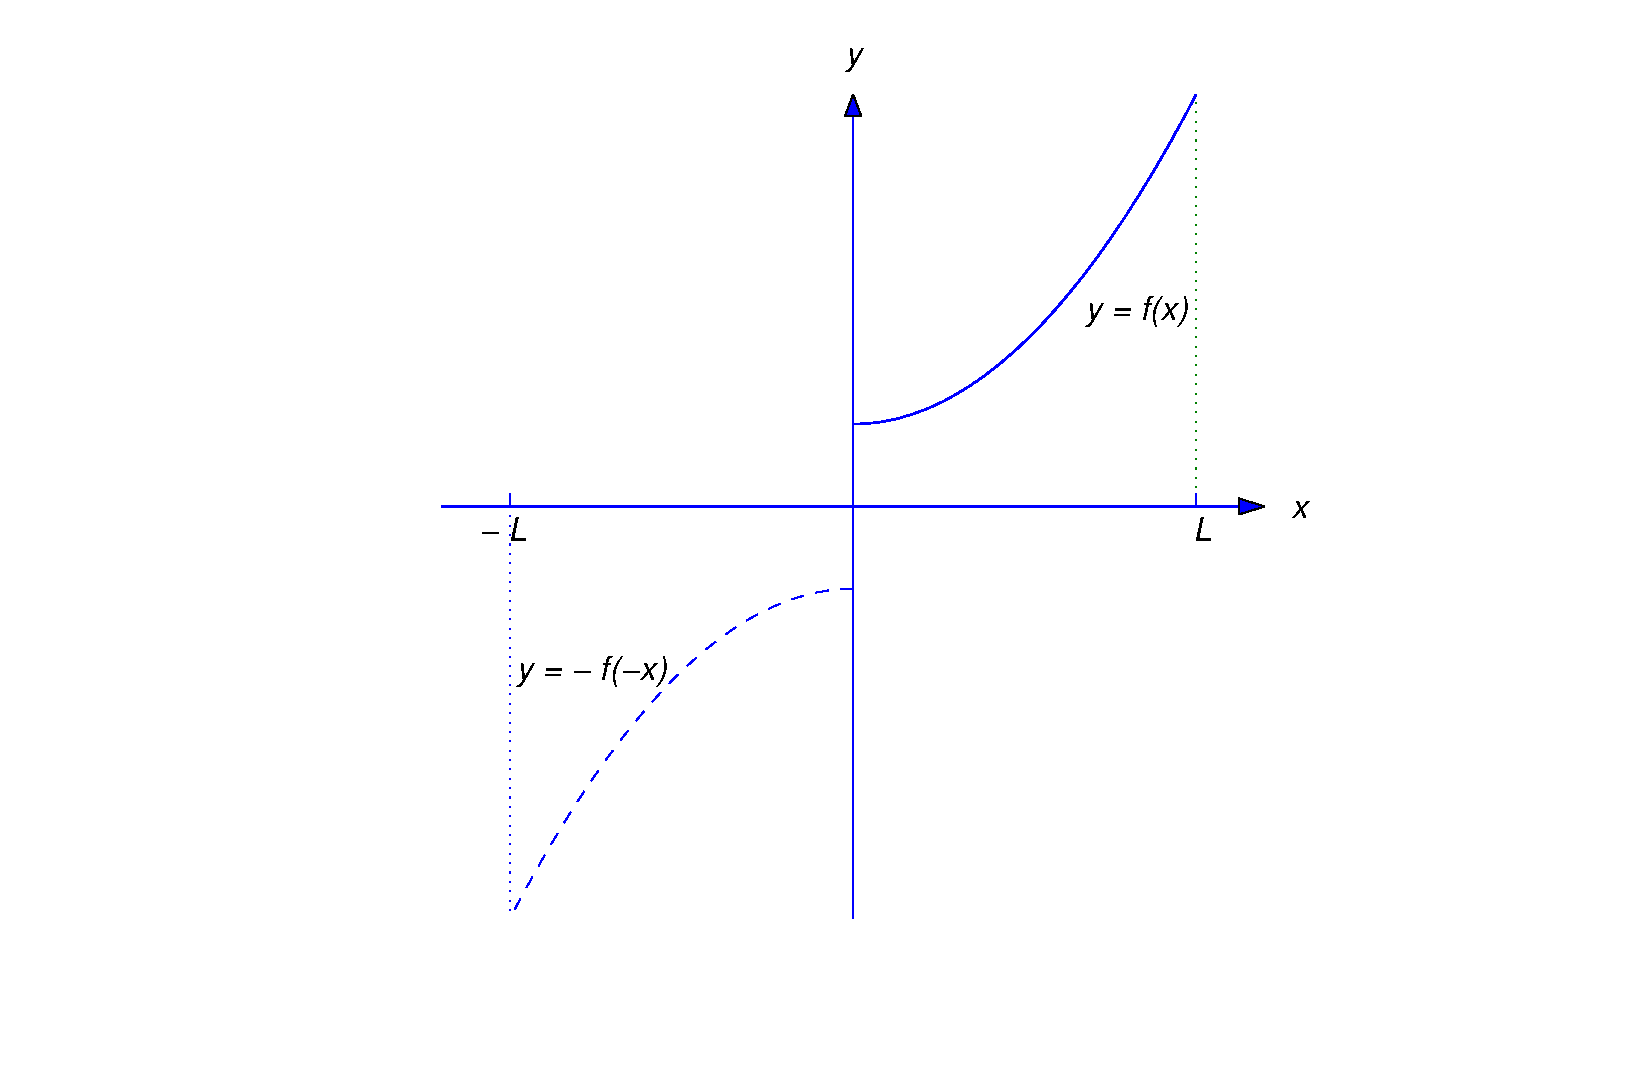
\includegraphics[bb=-78 148 689 643,width=5.67in,height=3.66in,keepaspectratio]{fig110302}
  \caption{}
  \label{figure:11.3.2}
\end{figure}

Applying
Theorem~11.2.4 to $f_2$ yields the next
theorem.

\begin{theorem}\color{blue} \label{thmtype:11.3.2}
If $f$ is piecewise smooth on $[0,L]$, then the Fourier sine series
$$
S(x)=\sum_{n=1}^\infty b_n\sin{n\pi x\over L}
$$
of $f$
on $[0,L]$,
with
$$
b_n={2\over L}\int_0^Lf(x)\sin{n\pi x\over L}\,dx,
$$
 converges for all $x$ in $[0,L]$; moreover,
$$
S(x)=
\left\{\begin{array}{cl}
0&\mbox{if }x=0  \\
f(x)&\mbox{if $0<x<L$ and $f$ is continuous at $x  $}\\[2\jot]
\dst{f(x-)+f(x+)\over2}&\mbox{if $0<x<L$ and $f$ is discontinuous at
$x  $}\\[2\jot]
0&\mbox{if }x=L.
\end{array}\right.
$$
\end{theorem}

\begin{example}\label{example:11.3.2} \rm
Find the Fourier sine series of $f(x)=x$ on $[0,L]$.
\end{example}

\solution
 The coefficients are
\begin{eqnarray*}
b_n&=&{2\over L}\int_0^Lx\sin{n\pi x\over L}\,dx
=-{2\over n\pi}\left[x\cos{n\pi x\over L}\lims0L-
\int_0^L
\cos{n\pi x\over L}\,dx\right]\\
&=& (-1)^{n+1}{2L\over n\pi}+{2L\over n^2\pi^2}\sin{n\pi x\over
L}\lims0L =(-1)^{n+1}{2L\over n\pi}.
\end{eqnarray*}
Therefore
$$
S(x)=\dst-{2L\over\pi}\sum_{n=1}^\infty{(-1)^n\over n}
\sin{n\pi x\over L}.
$$
Theorem~\ref{thmtype:11.3.2} implies that
$$
S(x)=
\left\{\begin{array}{cl}
x,&0\le x< L,\\0,& x=L.
\end{array}\right.
$$

\boxit{Mixed Fourier Cosine Series}

\noindent
From Exercise~11.1.~\hspace*{-3pt}\ref{exer:11.1.22}, the eigenfunctions
$$
 \cos{\pi x\over 2L},
\, \cos{3\pi x\over 2L},\dots,
 \, \cos{(2n-1)\pi x\over 2L},\dots
$$
 of the boundary value problem
\begin{equation} \label{eq:11.3.2}
y''+\lambda y=0,\quad y'(0)=0,\quad y(L)=0
\end{equation}
(Problem~4) are orthogonal on $[0,L]$.
 If $f$ is integrable on $[0,L]$ then the
Fourier expansion of $f$ in terms of these functions  is
$$
\sum_{n=1}^\infty c_n\cos{(2n-1)\pi x\over2L},
$$
where
$$
c_n={\dst\int_0^Lf(x)\cos{(2n-1)\pi x\over2L}\,dx\over\dst\int_0^L
\cos^2{(2n-1)\pi x\over L}\,dx}={2\over L}\int_0^Lf(x)\cos{(2n-1)\pi
x\over2L}\,dx.
$$

We'll  call this expansion the  {\color{blue}\it mixed Fourier cosine
series\/} of $f$ on $[0,L]$, because the boundary conditions
of (\ref{eq:11.3.2}) are ``mixed'' in that they require $y$
to be zero at
 one boundary point and $y'$ to be  zero at the other. By contrast,
the ``ordinary'' Fourier cosine series is associated with
(\ref{eq:11.3.1}), where the boundary conditions require that $y'$
be zero at both endpoints.

It can be shown (Exercise~\ref{exer:11.3.57}) that
 the mixed Fourier cosine series
of $f$ on $[0,L]$
is simply the restriction to  $[0,L]$ of the Fourier
cosine series  of
$$
f_3(x)=
\left\{\begin{array}{cl}
f(x),&0\le x\le L,\\-f(2L-x),&L< x\le 2L
\end{array}\right.
$$
on $[0,2L]$ (Figure~\ref{figure:11.3.3}).

\begin{figure}[H]
  \centering\color{blue}
  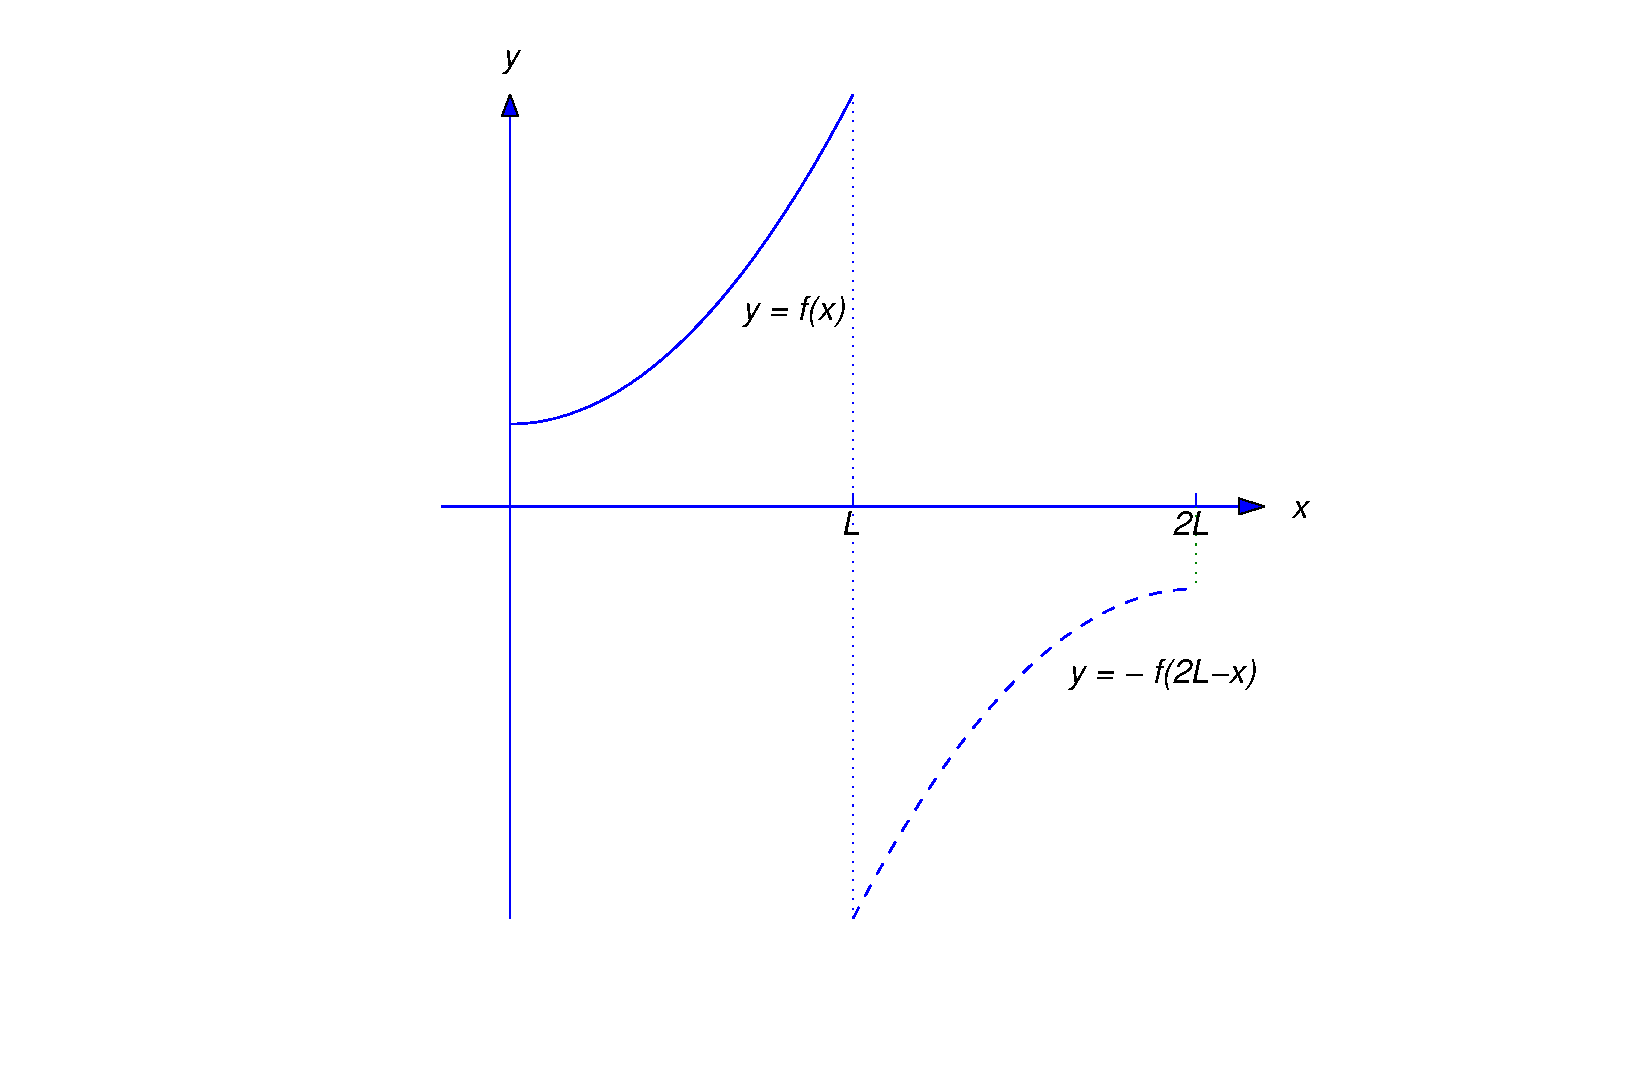
\includegraphics[bb=-78 148 689 643,width=5.67in,height=3.66in,keepaspectratio]{fig110303}
  \caption{}
  \label{figure:11.3.3}
\end{figure}

Applying  Theorem~\ref{thmtype:11.3.1}  with $f$ replaced by $f_3$ and $L$
replaced by $2L$ yields the next theorem.

\begin{theorem}\color{blue} \label{thmtype:11.3.3}
If  $f$ is piecewise smooth on $[0,L]$, then
the mixed Fourier cosine series
$$
C_M(x)=\sum_{n=1}^\infty c_n\cos{(2n-1)\pi x\over2L}
$$
of $f$ on $[0,L]$,
with
$$
c_n={2\over L}\int_0^Lf(x)\cos{(2n-1)\pi x\over2L}\,dx,
$$
 converges for all $x$ in $[0,L]$; moreover,
$$
C_M(x)=
\left\{\begin{array}{cl}
f(0+)&\mbox{if $x=0$}  \\
f(x)&\mbox{if $0<x<L$ and $f$ is continuous at $x$  }\\[2\jot]
\dst{f(x-)+f(x+)\over2}&\mbox{if $0<x<L$ and $f$ is discontinuous at
$x$  }\\[2\jot]
0&\mbox{if $x=L$.}
\end{array}\right.
$$
\end{theorem}

\begin{example}\label{example:11.3.3} \rm
Find  the mixed Fourier cosine series of
$f(x)=x-L$ on $[0,L]$.
\end{example}

\solution
 The coefficients are
\begin{eqnarray*}
c_n&=&{2\over L}\int_0^L(x-L)\cos{(2n-1)\pi x\over2L}\,dx\\
&=&{4\over(2n-1)\pi}\left[(x-L)\sin{(2n-1)\pi
x\over2L}\lims0L-\int_0^L
\sin{(2n-1)\pi x\over2L}\,dx\right]\\
&=&{8L\over(2n-1)^2\pi^2}
\cos{(2n-1)\pi x\over2L}\lims0L
=-{8L\over(2n-1)^2\pi^2}.
\end{eqnarray*}
Therefore
$$
C_M(x)=-{8L\over\pi^2}\sum_{n=1}^\infty{1\over(2n-1)^2}
\cos{(2n-1)\pi x\over2L}.
$$
Theorem~\ref{thmtype:11.3.3} implies that
$$
C_M(x)= x-L,\quad 0\le x\le L.
$$

\boxit{Mixed Fourier Sine Series}

\noindent
From  Exercise~11.1.~\hspace*{-3pt}\ref{exer:11.1.21},  the eigenfunctions
$$
 \sin{\pi x\over 2L},
\, \sin{3\pi x\over 2L},\dots,
 \, \sin{(2n-1)\pi x\over 2L},\dots
$$
of the boundary value problem
$$
y''+\lambda y=0,\quad y(0)=0,\quad y'(L)=0
$$
(Problem~3)   are orthogonal on $[0,L]$.
 If $f$ is integrable on $[0,L]$, then the
Fourier expansion of $f$ in terms of these functions
is
$$
\sum_{n=1}^\infty d_n\sin{(2n-1)\pi x\over2L},
$$
where
$$
d_n={\dst\int_0^Lf(x)\sin{(2n-1)\pi x\over2L}\,dx\over\dst\int_0^L
\sin^2{(2n-1)\pi x\over2L}\,dx}={2\over L}\int_0^Lf(x)\sin{(2n-1)\pi
x\over2L}\,dx.
$$
We'll  call this expansion the  {\color{blue}\it mixed Fourier sine
series\/} of $f$ on $[0,L]$.

It can be shown (Exercise~\ref{exer:11.3.58}) that
 the mixed Fourier sine series
of $f$ on $[0,L]$
is simply the restriction to  $[0,L]$ of the Fourier
sine series of
$$
f_4(x)=
\left\{\begin{array}{cl}
f(x),&0\le x\le L,\\f(2L-x),&L< x\le 2L,
\end{array}\right.
$$
on $[0,2L]$ (Figure~\ref{figure:11.3.4}).

\begin{figure}[H]
  \centering\color{blue}
  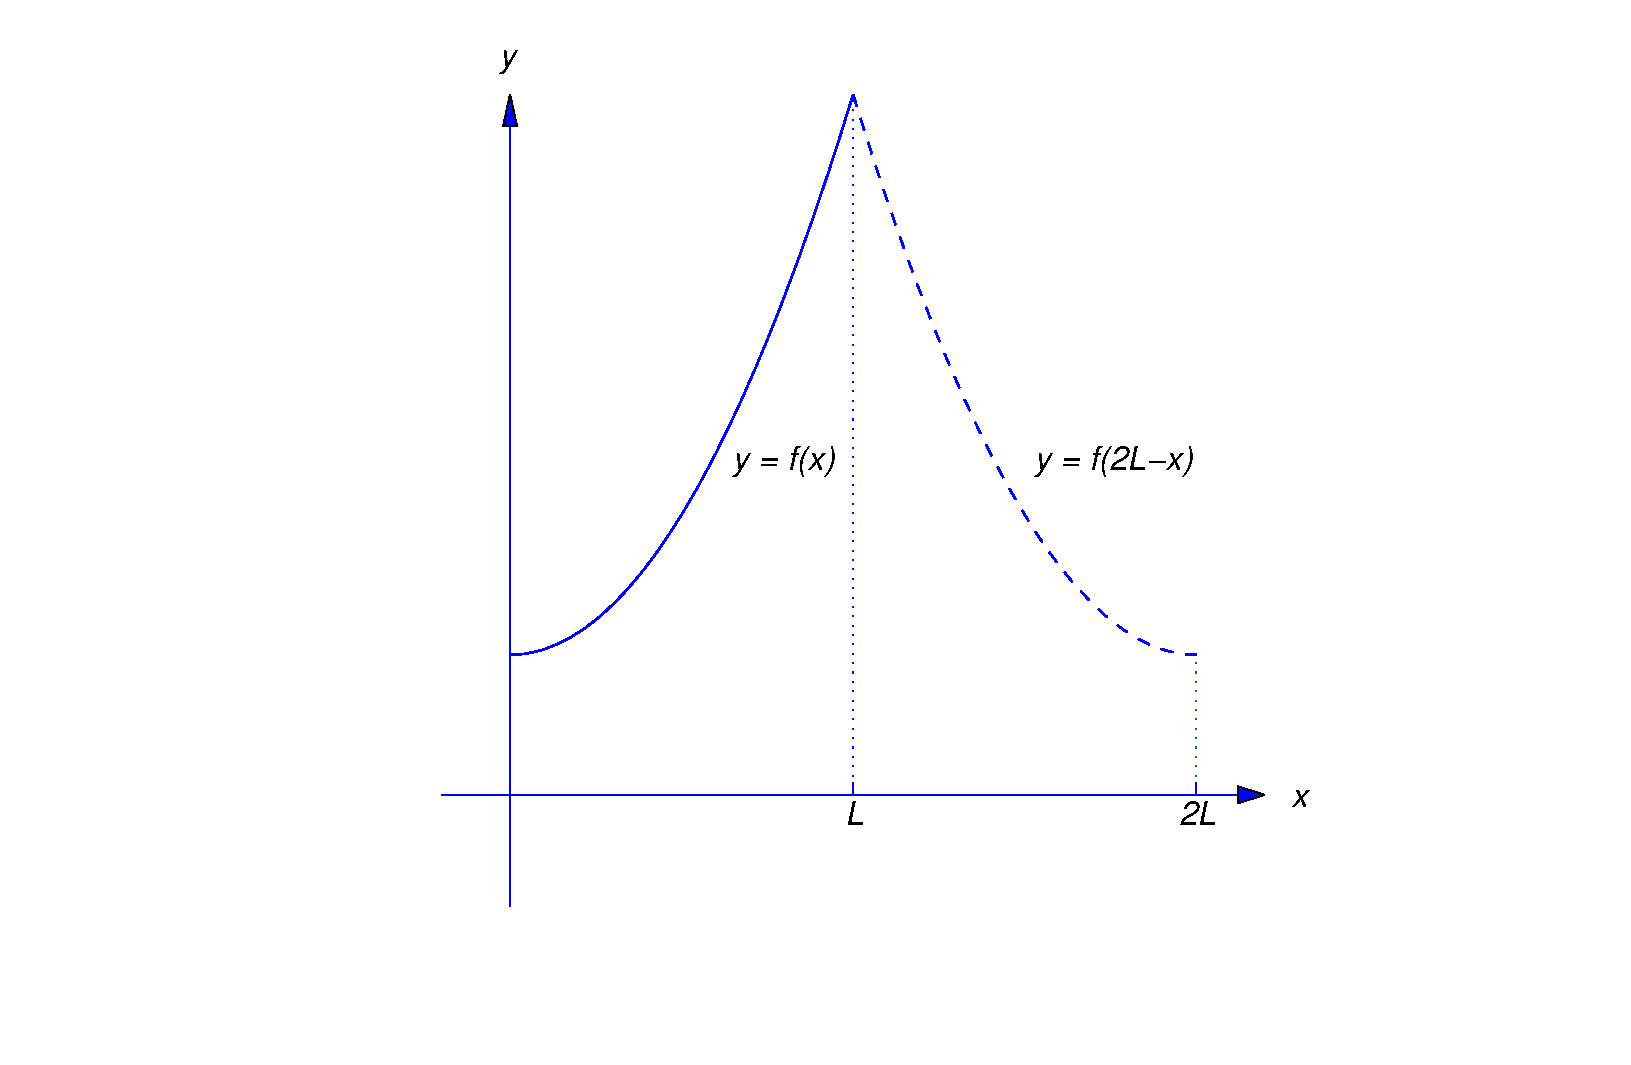
\includegraphics[bb=-78 148 689 643,width=5.67in,height=3.66in,keepaspectratio]{fig110304}
  \caption{}
  \label{figure:11.3.4}
\end{figure}

Applying Theorem~\ref{thmtype:11.3.2} with $f$ replaced by $f_4$ and $L$
replaced by $2L$ yields the next theorem.

\begin{theorem}\color{blue} \label{thmtype:11.3.4}
If $f$ is piecewise smooth on $[0,L]$, then the mixed Fourier
sine series
$$
S_M(x)=\sum_{n=1}^\infty d_n\sin{(2n-1)\pi x\over2L}
$$
of $f$ on $[0,L]$, with
$$
d_n={2\over L}\int_0^Lf(x)\sin{(2n-1)\pi x\over2L}\,dx,
$$
 converges for all $x$ in $[0,L]$; moreover,
$$
S_M(x)=
\left\{\begin{array}{cl}
0&\mbox{if $x=0$}  \\
f(x)&\mbox{if $0<x<L$ and $f$ is continuous at $x$  }\\[2\jot]
\dst{f(x-)+f(x+)\over2}&\mbox{if $0<x<L$ and $f$ is discontinuous at
$x$  }\\[2\jot]
f(L-)&\mbox{if $x=L$.}
\end{array}\right.
$$
\end{theorem}

\begin{example}\label{example:11.3.4} \rm
Find the mixed Fourier sine series of $f(x)=x$ on $[0,L]$.
\end{example}

\solution
 The coefficients are
\begin{eqnarray*}
d_n&=&{2\over L}\int_0^Lx\sin{(2n-1)\pi x\over2L}\,dx\\
&=&-{4\over(2n-1)\pi}\left[x\cos{(2n-1)\pi
x\over2L}\lims0L-
\int_0^L
\cos{(2n-1)\pi x\over2L}\,dx\right]\\
&=&{4\over(2n-1)\pi}
\int_0^L
\cos{(2n-1)\pi x\over2L}\,dx\\
&=&{8L\over(2n-1)^2\pi^2}\sin{(2n-1)\pi
x\over2L}\lims0L=(-1)^{n+1}{8L\over(2n-1)^2\pi^2}.
\end{eqnarray*}
Therefore
$$
S_M(x)=-{8L\over\pi^2}\sum_{n=1}^\infty{(-1)^n\over(2n-1)^2}
\sin{(2n-1)\pi x\over2L}.
$$
Theorem~\ref{thmtype:11.3.4} implies that
$$
S_M(x)=x,\quad 0\le x\le L.
$$

\boxit{A Useful Observation}

\noindent
In applications involving expansions in
terms of the eigenfunctions of Problems~1-4, the functions being
expanded
 are often  polynomials that  satisfy the boundary conditions
of the problem under consideration. In this case the next theorem
presents an
 efficient way  to obtain the
coefficients in the expansion.

\begin{theorem}\color{blue}  \label{thmtype:11.3.5}
\mbox{}\\

\part{a}
If $f'(0)=f'(L)=0$, $f''$ is continuous, and $f'''$ is piecewise
continuous  on $[0,L]$, then
\begin{equation} \label{eq:11.3.3}
f(x)=a_0+\sum_{n=1}^\infty a_n\cos{n\pi x\over L},
\quad 0\le x\le L,
\end{equation}
with
\begin{equation} \label{eq:11.3.4}
a_0={1\over L}\int_0^L f(x)\,dx \mbox{\quad and \quad}
a_n= {2L^2\over n^3\pi^3}\int_0^L f'''(x)\sin{n\pi
x\over L}\,dx,
\quad n\ge1.
\end{equation}

Now suppose $f'$ is continuous and $f''$ is piecewise
continuous on $[0,L]$.

\part{b}
If  $f(0)=f(L)=0$, then
$$
f(x)=\sum_{n=1}^\infty b_n\sin{n\pi x\over L},
\quad 0\le x\le L,
$$
with
\begin{equation} \label{eq:11.3.5}
b_n=-{2L\over n^2\pi^2}\int_0^L f''(x)\sin{n\pi
x\over L}\,dx.
\end{equation}

\part{c}
If  $f'(0)=f(L)=0$, then
$$
f(x)=
\sum_{n=1}^\infty c_n\cos{(2n-1)\pi x\over2L},
\quad 0\le x\le L,
$$
with
\begin{equation} \label{eq:11.3.6}
c_n=-{8L\over(2n-1)^2\pi^2}\int_0^L f''(x)\cos{(2n-1)\pi x\over2L}
\,dx.
\end{equation}

\part{d}
If  $f(0)=f'(L)=0$, then
$$
f(x)=
\sum_{n=1}^\infty d_n\sin{(2n-1)\pi x\over2L},
\quad 0\le x\le L,
$$
with
\begin{equation} \label{eq:11.3.7}
d_n=-{8L\over(2n-1)^2\pi^2}\int_0^L f''(x)\sin{(2n-1)\pi x\over2L}
\,dx.
\end{equation}
\end{theorem}

\proof  We'll prove \part{a} and leave the rest to you
(Exercises~\ref{exer:11.3.35}, \ref{exer:11.3.42}, and \ref{exer:11.3.50}).  Since
$f$ is continuous on
$[0,L]$, Theorem~\ref{thmtype:11.3.1} implies (\ref{eq:11.3.3}) with $a_0$,
$a_1$, $a_2$,... as defined in Theorem~\ref{thmtype:11.3.1}. We already
know that
$a_0$ is as in
(\ref{eq:11.3.4}). If  $n\ge1$, integrating twice by parts yields
\begin{eqnarray*}
a_n&=& {2\over L}\int_0^L f(x)\cos{n\pi x\over L}\,dx\\
&=&{2\over n\pi}\left[f(x)\sin{n\pi x\over L}\lims0L
-\int_0^Lf'(x)\sin{n\pi x\over L}\,dx\right]\\
&=&-{2\over n\pi}
\int_0^Lf'(x)\sin{n\pi x\over L}\,dx
\mbox{ (since $\sin0=\sin n\pi=0$)}\\
&=&{2L\over n^2\pi^2}\left[f'(x)\cos{n\pi x\over L}\lims0L
-\int_0^Lf''(x)\cos{n\pi x\over L}\right]\,dx\\
&=&
-{2L\over n^2\pi^2}\int_0^Lf''(x)\cos{n\pi x\over L}\,dx
\mbox{ (since $f'(0)=f'(L)=0$)}\\
&=&-{2L^2\over n^3\pi^3}\left[f''(x)\sin{n\pi x\over L}\lims0L
-\int_0^Lf'''(x)\sin{n\pi x\over L}\,dx\right]\\
&=&
{2L^2\over n^3\pi^3}\int_0^Lf'''(x)\sin{n\pi x\over L}\,dx
\mbox{ (since $\sin0=\sin n\pi=0$).}
\end{eqnarray*}
(By an argument similar to one used in the proof of Theorem~8.3.1,
 the last integration by parts is legitimate
in the case where $f'''$ is undefined at finitely many points in
$[0,L]$, so long as it's piecewise continuous on $[0,L]$.)
This completes the proof.

\begin{example}\label{example:11.3.5} \rm
Find the Fourier cosine expansion of $f(x)=x^2(3L-2x)$
on $[0,L]$.
\end{example}

\solution
Here
$$
a_0={1\over L}\int_0^L(3Lx^2-2x^3)\,dx={1\over
L}\left(Lx^3-{x^4\over2}
\right)\lims0L={L^3\over2}
$$
and
$$
a_n={2\over L}\int_0^L(3Lx^2-2x^3)\cos{n\pi x\over L}\,dx,\quad n\ge1.
$$
Evaluating this integral directly is laborious.
However, since $f'(x)=6Lx-6x^2$, we see that $f'(0)=f'(L)=0$.
Since $f'''(x)=-12$, we see from (\ref{eq:11.3.4}) that if $n\ge1$ then
\begin{eqnarray*}
a_n&=&-{24L^2\over n^3\pi^3}\int_0^L\sin{n\pi x\over L}\,dx
={24L^3\over n^4\pi^4}\cos{n\pi x\over L}\lims0L={24L^3\over
n^4\pi^4}[(-1)^n-1]\\
&=&
\left\{\begin{array}{cl}
\dst-{48L^3\over(2m-1)^4\pi^4}&\mbox{if  $n=2m-1$},\\
0&\mbox{if $n=2m$.}
\end{array}\right.
\end{eqnarray*}
Therefore
$$
C(x)={L^3\over2}-{48L^3\over\pi^4}\sum_{n=1}^\infty{1\over
(2n-1)^4}\cos{(2n-1)\pi x\over L}.
$$

\begin{example}\label{example:11.3.6} \rm
Find the Fourier sine expansion of
$f(x)=x(x^2-3Lx+2L^2)$
on $[0,L]$.
\end{example}

\solution
Since $f(0)=f(L)=0$ and $f''(x)=6(x-L)$, we see from (\ref{eq:11.3.5})
that
\begin{eqnarray*}
b_n&=&-
{12L\over n^2\pi^2}\int_0^L(x-L)\sin{n\pi x\over L}\,dx\\
&=&{12L^2\over n^3\pi^3}\left[(x-L)\cos{n\pi x\over L}\lims0L
-\int_0^L\cos{n\pi x\over L}\,dx\right]\\
&=&{12L^2\over n^3\pi^3}\left[L-\frac{L}{n\pi}\sin\frac{n\pi
x}{L}\lims0L\right]
={12L^3\over
n^3\pi^3}.
\end{eqnarray*}
Therefore
$$
S(x)=\dst{12L^3\over\pi^3}\sum_{n=1}^\infty{1\over n^3}
\sin{n\pi x\over L}.
$$

\begin{example}\label{example:11.3.7} \rm
Find  the mixed Fourier cosine expansion of
$f(x)=3x^3-4Lx^2+L^3$
on $[0,L]$.
\end{example}

\solution
Since $f'(0)=f(L)=0$ and $f''(x)=2(9x-4L)$, we see from (\ref{eq:11.3.6})
that
\begin{eqnarray*}
c_n&=&
-{16L\over(2n-1)^2\pi^2}
\int_0^L(9x-4L)\cos{(2n-1)\pi x\over2L}\,dx\\
&=&-{32L^2\over(2n-1)^3\pi^3}\left[(9x-4L)\sin{(2n-1)\pi x\over2L}
\lims0L-9\int_0^L\sin{(2n-1)\pi x\over2L}\right]\,dx\\
&=&-{32L^2\over(2n-1)^3\pi^3}
\left[(-1)^{n+1}5L+{18L\over(2n-1)\pi}\cos{(2n-1)\pi x\over2L}
\lims0L\right] \\
&=&{32L^3\over(2n-1)^3\pi^3}
\left[(-1)^n5+{18\over(2n-1)\pi}\right].
\end{eqnarray*}
Therefore
$$
C_M(x)=\dst{32L^3\over\pi^3}\sum_{n=1}^\infty{1\over(2n-1)^3}\left[
(-1)^n5+{18\over(2n-1)\pi}\right]\cos{(2n-1)\pi
x\over2L}.
$$

\begin{example}\label{example:11.3.8} \rm
Find  the mixed Fourier  sine expansion of
$$
f(x)=x(2x^2-9Lx+12L^2)
$$
on $[0,L]$.
\end{example}

\solution
Since $f(0)=f'(L)=0$, and $f''(x)=6(2x-3L)$, we see from (\ref{eq:11.3.7})
that
\begin{eqnarray*}
d_n&=&-\dst{48L\over(2n-1)^2\pi^2}\int_0^L(2x-3L)
\sin{(2n-1)\pi x\over2L}\,dx\\
&=&\dst{96L^2\over(2n-1)^3\pi^3}\left[(2x-3L)\cos{(2n-1)\pi
x\over2L}\lims0L-2\int_0^L\cos{(2n-1)\pi x\over2L}\,dx\right]\\
&=&\dst{96L^2\over(2n-1)^3\pi^3}\left[3L-{4L\over(2n-1)\pi}
\sin{(2n-1)\pi x\over2L}\lims0L\right]\\
&=&\dst{96L^3\over(2n-1)^3\pi^3}\left[3+(-1)^n{4\over(2n-1)\pi}\right].
\end{eqnarray*}
Therefore
$$
S_M(x)
=\dst{96L^3\over\pi^3}\sum_{n=1}^\infty
{1\over(2n-1)^3}\left[3+(-1)^n{4\over(2n-1)\pi}\right]\sin{(2n-1)\pi
x\over2L}.
$$

\exercises
\noindent
In exercises marked by \Cex\, graph $f$
and some partial sums of the required series. If the interval
is $[0,L]$, choose a specific value of $L$ for the graph.

\noindent
\emph{In Exercises~\ref{exer:11.3.1}-\ref{exer:11.3.10} find the Fourier
cosine series.}

\begin{exerciselist}

\item\label{exer:11.3.1}
$f(x)=x^2$;  \quad $[0,L]$

\item\label{exer:11.3.2}
\Cex $f(x)=1-x$;   \quad $[0,1]$

\item\label{exer:11.3.3} \Cex
$f(x)=x^2-2Lx$;   \quad $[0,L]$

\item\label{exer:11.3.4}
$f(x)=\sin kx$\, ($k\ne$ integer);\quad    $[0,\pi]$

\item\label{exer:11.3.5} \Cex
$f(x)=
\left\{\begin{array}{cl}
1,&0\le x\le{L\over2}\\0,&{L\over2}<x<L;
\end{array}\right.$ \quad $[0,L]$

\item\label{exer:11.3.6}
$f(x)=x^2-L^2$;   \quad $[0,L]$

\item\label{exer:11.3.7}
 $f(x)=(x-1)^2$;  \quad $[0,1]$

\item\label{exer:11.3.8}
$f(x)=e^x$;   \quad $[0,\pi]$

\item\label{exer:11.3.9} \Cex
$f(x)=x(L-x)$;  \quad $[0,L]$

\item\label{exer:11.3.10} \Cex
$f(x)=x(x-2L)$;  \quad $[0,L]$

\exercisetext{
In Exercises~\ref{exer:11.3.11}-\ref{exer:11.3.17} find the Fourier sine
series.}

\item\label{exer:11.3.11}  \Cex
$f(x)=1$;  \quad$[0,L]$

\item\label{exer:11.3.12}
\Cex $f(x)=1-x$;   \quad $[0,1]$

\item\label{exer:11.3.13}
$f(x)=\cos kx$\, ($k\ne$ integer);  \quad $[0,\pi]$

\item\label{exer:11.3.14} \Cex
$f(x)=
\left\{\begin{array}{cl}
1,&0\le x\le{L\over2}\\0,&{L\over2}<x<L;
\end{array}\right.$ \quad $[0,L]$

\item\label{exer:11.3.15} \Cex
$f(x)=
\left\{\begin{array}{cl}
x,&0\le x\le{L\over2},\\L-x,&{L\over2}\le x\le L;
\end{array}\right.$
\quad $[0,L]$.

\item\label{exer:11.3.16} \Cex
$f(x)=x\sin x$;   \quad $[0,\pi]$

\item\label{exer:11.3.17}
$f(x)=e^x$;   \quad $[0,\pi]$

\exercisetext{
In Exercises~\ref{exer:11.3.18}-\ref{exer:11.3.24} find the mixed Fourier
cosine series.}

\item\label{exer:11.3.18}  \Cex
$f(x)=1$;  \quad$[0,L]$

\item\label{exer:11.3.19}
$f(x)=x^2$;  \quad $[0,L]$

\item\label{exer:11.3.20}
\Cex $f(x)=x$;   \quad $[0,1]$

\item\label{exer:11.3.21} \Cex
$f(x)=
\left\{\begin{array}{cl}
1,&0\le x\le{L\over2}\\0,&{L\over2}<x<L;
\end{array}\right.$ \quad $[0,L]$

\item\label{exer:11.3.22}
$f(x)=\cos x$;   \quad $[0,\pi]$

\item\label{exer:11.3.23}
$f(x)=\sin x$;   \quad $[0,\pi]$

\item\label{exer:11.3.24} \Cex
$f(x)=x(L-x)$;  \quad $[0,L]$

\exercisetext{
In Exercises~\ref{exer:11.3.25}-\ref{exer:11.3.30} find the mixed Fourier sine
series.}

\item\label{exer:11.3.25}  \Cex
$f(x)=1$;  \quad$[0,L]$

\item\label{exer:11.3.26}
$f(x)=x^2$;  \quad $[0,L]$

\item\label{exer:11.3.27} \Cex
$f(x)=
\left\{\begin{array}{cl}
1,&0\le x\le{L\over2}\\0,&{L\over2}<x<L;
\end{array}\right.$\quad  $[0,L]$

\item\label{exer:11.3.28}
$f(x)=\cos x$;   \quad $[0,\pi]$

\item\label{exer:11.3.29}
$f(x)=\sin x$;   \quad $[0,\pi]$

\item\label{exer:11.3.30} \Cex
$f(x)=x(L-x)$;  \quad $[0,L]$.

\exercisetext{In Exercises~\ref{exer:11.3.31}-\ref{exer:11.3.34}
use Theorem~\ref{thmtype:11.3.5}\part{a} to find the  Fourier
cosine series of $f$ on~$[0,L]$.}

\item\label{exer:11.3.31}
$f(x)=3x^2(x^2-2L^2)$

\item\label{exer:11.3.32}
$f(x)=x^3(3x-4L)$

\item\label{exer:11.3.33}
$f(x)=x^2(3x^2-8Lx+6L^2)$

\item\label{exer:11.3.34}
$f(x)=x^2(x-L)^2$

\item\label{exer:11.3.35}
\begin{alist}
\item % (a)
Prove Theorem~\ref{thmtype:11.3.5}\part{b}.
\item % (b)
In addition to the assumptions of Theorem~\ref{thmtype:11.3.5}\part{b},
suppose  $f''(0)=f''(L)=0$, $f'''$ is continuous,  and $f^{(4)}$
is piecewise continuous on $[0,L]$.
Show that
$$
b_n={2L^3\over n^4\pi^4}\int_0^L f^{(4)}(x)\sin{n\pi
x\over L}\,dx,
\quad n\ge1.
$$
\end{alist}

\exercisetext{
In Exercises~\ref{exer:11.3.36}-\ref{exer:11.3.41}
use Theorem~\ref{thmtype:11.3.5}\part{b}
or, where applicable,
Exercise~$11.1$.~\hspace*{-3pt}\ref{exer:11.3.35}\part{b},
to find the Fourier sine series of $f$  on $[0,L]$.}

\item\label{exer:11.3.36}
\Cex $f(x)=x(L-x)$

\item\label{exer:11.3.37}
\Cex\quad$f(x)=x^2(L-x)$

\item\label{exer:11.3.38}
$f(x)=x(L^2-x^2)$

\item\label{exer:11.3.39}
$f(x)=x(x^3-2Lx^2+L^3)$

\item\label{exer:11.3.40}
$f(x)=x(3x^4-10L^2x^2+7L^4)$

\item\label{exer:11.3.41}
$f(x)=x(3x^4-5Lx^3+2L^4)$

\item\label{exer:11.3.42}
\begin{alist}
\item % (a)
Prove Theorem~\ref{thmtype:11.3.5}\part{c}.
\item % (b)
In addition to the assumptions of Theorem~\ref{thmtype:11.3.5}\part{c},
suppose
$f''(L)=0$, $f''$ is continuous, and $f'''$ is piecewise continuous on
$[0,L]$. Show that
$$
c_n={16L^2\over(2n-1)^3\pi^3}\int_0^L f'''(x)\sin{(2n-1)\pi x\over2L}
\,dx,\quad n\ge1.
$$
\end{alist}

\exercisetext{
In Exercises~\ref{exer:11.3.43}-\ref{exer:11.3.49}
use Theorem~\ref{thmtype:11.3.5}\part{c}
or, where applicable,
Exercise~$11.1$.~\hspace*{-3pt}\ref{exer:11.3.42}\part{b},
to find the mixed Fourier
cosine series of $f$ on $[0,L]$.}

\item\label{exer:11.3.43}
\Cex $f(x)=x^2(L-x)$

\item\label{exer:11.3.44}
$f(x)=L^2-x^2$

\item\label{exer:11.3.45}
$f(x)=L^3-x^3$

\item\label{exer:11.3.46}
$f(x)=2x^3+3Lx^2-5L^3$

\item\label{exer:11.3.47}
$f(x)=4x^3+3Lx^2-7L^3$

\item\label{exer:11.3.48}
$f(x)=x^4-2Lx^3+L^4$

\item\label{exer:11.3.49}
$f(x)=x^4-4Lx^3+6L^2x^2-3L^4$

\item\label{exer:11.3.50}
\begin{alist}
\item % (a)
Prove Theorem~\ref{thmtype:11.3.5}\part{d}.
\item % (b)
In addition to the assumptions of Theorem~\ref{thmtype:11.3.5}\part{d},
suppose
$f''(0)=0$, $f''$ is continuous, and $f'''$ is piecewise continuous on
$[0,L]$. Show that
$$
d_n=-{16L^2\over(2n-1)^3\pi^3}\int_0^L f'''(x)\cos{(2n-1)\pi x\over2L}
\,dx,\quad n\ge1.
$$
\end{alist}

\exercisetext{In Exercises~\ref{exer:11.3.51}-\ref{exer:11.3.56}
use Theorem~\ref{thmtype:11.3.5}\part{d} or, where applicable,
Exercise~\ref{exer:11.3.50}\part{b}, to find the mixed Fourier sine series
of the $f$ on $[0,L]$.}

\item\label{exer:11.3.51}
$f(x)=x(2L -x)$

\item\label{exer:11.3.52}
$f(x)=x^2(3L-2x)$

\item\label{exer:11.3.53}
 $f(x)=(x-L)^3+L^3$

\item\label{exer:11.3.54}
 $f(x)=x(x^2-3L^2)$

\item\label{exer:11.3.55}
$f(x)=x^3(3x-4L)$

\item\label{exer:11.3.56}
 $f(x)=x(x^3-2Lx^2+2L^3)$

\item\label{exer:11.3.57}
Show that the mixed Fourier cosine series of $f$ on $[0,L]$ is the
restriction to $[0,L]$ of the Fourier cosine series of
$$
f_3(x)=
\left\{\begin{array}{cl}
f(x),&0\le x\le L,\\-f(2L-x),&L< x\le 2L
\end{array}\right.
$$
on $[0,2L]$.  Use this to prove Theorem~\ref{thmtype:11.3.3}.

\item\label{exer:11.3.58}
Show that the mixed Fourier sine series of $f$ on $[0,L]$ is the
restriction to $[0,L]$ of the Fourier sine series of
$$
f_4(x)=
\left\{\begin{array}{cl}
f(x),&0\le x\le L,\\f(2L-x),&L< x\le 2L
\end{array}\right.
$$
on $[0,2L]$.  Use this to prove Theorem~\ref{thmtype:11.3.4}.

\item\label{exer:11.3.59}
Show that the Fourier sine series of $f$ on $[0,L]$ is the restriction
to $[0,L]$ of the Fourier sine series of
$$
f_3(x)=
\left\{\begin{array}{cl}
f(x),&0\le x\le L,\\-f(2L-x),&L< x\le 2L
\end{array}\right.
$$
on $[0,2L]$.

\item\label{exer:11.3.60}
Show that  the Fourier cosine series
of $f$ on $[0,L]$
 is the restriction
to $[0,L]$ of the Fourier cosine series of
$$
f_4(x)=
\left\{\begin{array}{cl}
f(x),&0\le x\le L,\\f(2L-x),&L< x\le 2L
\end{array}\right.
$$
on  $[0,2L]$.

\end{exerciselist}


